%\documentclass[10pt,twocolumn,journal]{IEEEtran}
%\documentclass[12pt,draftclsnofoot,onecolumn,journal]{IEEEtran}
\documentclass[10pt, conference]{IEEEtran}
\usepackage[english]{babel}
\usepackage{url}
\usepackage{cite}
%\usepackage[noadjust]{cite}
\usepackage{epsf}
\usepackage{amssymb,amsmath,amsfonts}
\usepackage{array}
\usepackage{graphics}
\usepackage{graphicx}
\usepackage{cleveref}
\usepackage{theorem}
\usepackage{algorithm}
\usepackage{algorithmic}
\usepackage{caption}
\usepackage[table]{xcolor}
%\usepackage{subcaption}
\usepackage{soul}
\usepackage{subfig}
\usepackage{minted}
\usepackage{adjustbox}
%\usepackage{color}
%\usepackage[symbol]{footmisc}
\usepackage[para]{footmisc}
%\usepackage{changes}
\usepackage[final]{changes}
%\usepackage{lineno}
%\linenumbers
\renewcommand{\thefootnote}{\fnsymbol{footnote}}
\newcommand{\smartparagraph}[1]{\vspace{.05in}\noindent\textbf{#1}}
\PassOptionsToPackage{bookmarks=false}{hyperref}

\pagestyle{empty}



%\def\symbolfootnote[#1]#2{\begingroup
%\def\thefootnote{\fnsymbol{footnote}}
%\footnote[#1]{#2}\endgroup}

%\IEEEoverridecommandlockouts
%\IEEEpubid{\makebox[\columnwidth]{978-1-7281-5684-2/20/\$31.00~\copyright{}2020 IEEE \hfill} \hspace{\columnsep}\makebox[\columnwidth]{ }}

\begin{document}

\title{Field trial of programmable L3 VPN service deployment using SDN-Based Multi-domain Service Provisioning over IP/Optical networks}

\author{
\IEEEauthorblockN{Samier Barguil\IEEEauthorrefmark{1}, Victor Lopez\IEEEauthorrefmark{2}, Cristyan Manta-Caro\IEEEauthorrefmark{4}, Arturo Mayoral Lopez De Lerma\IEEEauthorrefmark{2},\\
Oscar Gonzalez De Dios\IEEEauthorrefmark{2}, Edward Echeverry\IEEEauthorrefmark{3}, Juan Pedro Fernandez-Palacios\IEEEauthorrefmark{2}, Janne Karvonen\IEEEauthorrefmark{5},\\
Jutta Kemppainen\IEEEauthorrefmark{5}, Natalia Maya\IEEEauthorrefmark{5}, and Ricard Vilalta\IEEEauthorrefmark{6}}
\IEEEauthorblockA{
\IEEEauthorrefmark{1}Universidad Autonoma de Madrid, Madrid, Spain\\
\IEEEauthorrefmark{2}Telefonica I+D, Ronda de la Comunicacion, Madrid, Spain \\
\IEEEauthorrefmark{3}Telefonica Movistar, Transversal 60 No 114ª -55. Bogotá, Colombia\\
\IEEEauthorrefmark{4}Wipro Technologies Ltd., Doddakannelli, Sarjapur Road
Bengaluru - 560 035, India\\
\IEEEauthorrefmark{5}Infinera Corporation, 140 Caspian Court, Sunnyvale, CA 94089, USA\\
\IEEEauthorrefmark{6}Centre Tecnol\`{o}gic de Telecomunicacions de Catalunya (CTTC/CERCA), Castelldefels, Spain}

}

\maketitle

\begin{abstract}
%Software-Defined Networking (SDN) is a powerful paradigm already transforming the everyday operations in Telecommunications Networks. SDN came with the idea of decoupling forwarding and control plane in the switches via OpenFlow, but it has evolved to cope with the needs of production networks. 
Network operators can not change their footprint to upgrade the entire Network to support SDN from scratch. \replaced{Hence,}{This why} network operators adapt\added{ed} the original SDN concept into a hybrid SDN approach to have a pragmatic, evolutionary, and economically viable solution. This paper tests an SDN architecture based on a hierarchical structure of a Software-Defined Transport Networking (SDTN) controller, which deals with the end-to-end service provision and topology collection on top of a set of SDN controllers for each technological domain. The authors demonstrate L3/L2 VPN service deployment using an underlay multi-domain IP/Optical networks in a field trial. The approach allows a service provider to migrate brownfield scenarios into SDN domains using programmatic interfaces.

%network islands into SDN domains using programmatic interfaces.

%Service provisioning is a key process in the value chain for supplying next-generation services to customers of all sizes and characteristics. Commonly, during years service provisioning was executed manually, then supported by service activators tuned tools for the vendor- specific combination of network elements. With the advent boom of SDN, service delivery operations can be performed in an agnostic-vendor fashion using standard data models and protocols. However, new challenges still persist such as orchestrate multiple layers required for covering long-haul, medium and short distances. Multidomain networking between IP/MPLS-based layers and underlying WDM multi-layer technologies require further coordination and orchestration. This presents two use cases to enable multidomain service provisioning and the corresponding topology visualization. Moreover, this work demonstrates the capabilities of a SDTN controller in a field trial environment our approach for Hybrid SDN architectures.
\end{abstract}

%\begin{IEEEkeywords}
%Security SLA, NFV, orchestration, V2X, C-ITS, CAM, DENM, ACCA
%\end{IEEEkeywords}

%\vspace{-0.2in}

\section{Introduction}
Software-Defined Networking (SDN) has emerged as the new reference paradigm to promote network automation and programmability. It has promoted the idea of a radical transformation in all aspects of the: service delivery, network, and traffic management; because end-to-end automatic service provision, automated monitoring, fast issue detection, and event-based decision taking are mandatory functionalities to offer a high-quality customer experience \cite{ordonez2017network}.

Conceptually, SDN allows a full decoupling between control and forwarding plane on Physical Network Functions (PNFs). 
This concept allows the centralization of complex processing tasks and enables integrating white boxes (i.e., smaller equipment, high port density, low processing capacity, \replaced{made}{facts} with generic hardware, and lower production cost) in the network access layers. However, this promise is still not a reality on the service provider networks. Although the term SDN seems new, it has already been more than twelve (12) years since a Stanford team defined OpenFlow and founded NICIRA (NICIRA was the first company to develop a commercial SDN controller (NOX)). Nowadays, despite millionaire investments and several SDN controller solutions available \cite{medved2014opendaylight,berde2014onos} on the market, almost no service provider has a full operative SDN network controller deployed. Some of the main barriers found by service providers until now are:

\begin{itemize}
    \item There are still many dependencies on manually executing tasks.
    \item Network control tasks can not be fully centralized.
    \item The stack of protocols deployed in the network is very complicated.  The knowledge that network operators require to solve problems continues to be very specific.
    \item Confidence in automation solutions is not very high.
    \item Many networks have grown via company acquisitions. In many cases internally they operate as independent carriers. 
    \item Standardization is not complete, generating a lack of full interoperability between vendors.
\end{itemize}

Several new approaches have been gradually released in recent years to adopt SDN as a hybrid solution in brownfield scenarios. Some of the most promising methods were defined using agile methodologies, as software development and IT operations (DevOps) solutions \cite{choi2018agile}. 
These agile methodologies usually take a small network task and solve it using a programmatic approach. It allows the simple and more frequent integration of new functionalities. Network provisioning is one of the recurrent tasks selected for agile automation; because it is a diary job that includes the usage of well-defined templates to deploy MPLS-based services on the network.

The Layer 3 Virtual Private Network (VPN) service defined in RFC 4364 \cite{rfc4364} provides a multi-point, routed service to a customer over an IP/MPLS core. L3VPNs are widely used in carrier-grade networks to deploy 3G/4G, fixed, and enterprise services. Traffic policies can be applied in these services to reuse the same transport network, and it also makes it feasible to combine access technologies over an MPLS core. On the other hand, L2 services belong to the class of IP virtual leased line (VLL) services or virtual private LAN (VPLS) services \cite{andersson2006framework}, which are a fundamental part of the service portfolio offered by service providers. 

This work proves the viability of the implementations of programmable network interfaces for the deployment of L2/L3 services in IP over optical networks using common standard models and protocols. A field trial including multiple network controllers (two for IP/MPLS and two for DWDM) and a real-commercial-multivendor-operative network was installed by Telefonica in their premises in Colombia to validate the concept.

The paper is structured as follows: \Cref{sec:soa} provides a review of the State of the Art both on the provisioning of automated L2/L3 VPN services. \Cref{section:arq} describes the SDN reference architecture and details the principles of the network programmability, including concepts of YANG and used protocols. Then, Section \ref{section:trial} details the test architecture, including commercial network controllers and the results obtained in this implementation. Finally, conclusions and perspectives are drawn in \Cref{section:conclusions}.    

\added{
The list of abbreviations and its definition is defined in \cref{tab:abbreviations}.}

\begin{table}[htb!]
\caption{List of abbreviations used across the document}
\label{tab:abbreviations}
\begin{tabular}{|l|l|}
\hline
Abbreviation & \multicolumn{1}{c|}{Definition}              \\ \hline
API          & Application programming interface            \\ \hline
BGP          & Border Gateway Protocol                      \\ \hline
BGP-LS       & Border Gateway Protocol Link-State            \\ \hline
BSS          & Business Support Systems                     \\ \hline
CE           & Customer Edge                                \\ \hline
CRUD         & Create, Read, Update and Delete              \\ \hline
DWDM         & Dense Wavelength Division Multiplexing       \\ \hline
GMPLS        & General Multi-Protocol Label Switching       \\ \hline
GUI          & Graphical user interface                     \\ \hline
IETF         & Internet Engineering Task Force              \\ \hline
IGP          & Interior Gateway Protocol                    \\ \hline
IP           & Internet Protocol                            \\ \hline
L2           & Layer-2                                      \\ \hline
L2SM         & L2VPN Service Model                          \\ \hline
L2SM         & L2VPN Service Model                          \\ \hline
L2NM         & L2VPN Network Model                          \\ \hline
L3           & Layer-3                                      \\ \hline
L3SM         & L3VPN Service Model                          \\ \hline
L3NM         & L3VPN Network Model                          \\ \hline
LAG          & Link aggregation group                       \\ \hline
LDP          & Label Distribution Protocol                  \\ \hline
MPLS         & Multiprotocol Label Switching                \\ \hline
NBI          & Northbound interface                         \\ \hline
ONF          & Open Networking Foundation                   \\ \hline
OSS          & Operation Support Systems                    \\ \hline
PCE          & Path Computation Element                     \\ \hline
PE           & Provider Edge                                \\ \hline
QoS          & Quality of service                           \\ \hline
RD           & Route Distinguisher                          \\ \hline
RPC          & Remote Procedure Call                        \\ \hline
RT           & Route Target                                 \\ \hline
SBI          & South Bound Interface                        \\ \hline
SDN          & Software Defined Network                     \\ \hline
SDNc         & Software Defined Network Controller          \\ \hline
SDTN         & Software Defined Transport Network           \\ \hline
TAPI         & Transport API                                \\ \hline
URI          & Uniform resource identifier                  \\ \hline
VPN          & Virtual Private Network                      \\ \hline
VRF          & Virtual Routing and Forwarding               \\ \hline
YANG         & Yet Another Next Generation                   \\ \hline
\end{tabular}
\end{table}

\section{State of the Art}
\label{sec:soa}

The IP service models are YANG modules defined to support the creation, deletion, and retrieval of L3/L2VPN services and the IP/MPLS network topology collection. The models used in this work are abstract models that technologically describe the network requirements and are RFCs or working-group-drafts inside the IETF.

\subsubsection{L3VPN Service Model (L3SM)}
\label{section:l3nm}
Multi-Protocol Label Switching (MPLS) Virtual Private Networks (VPNs) have seen an unparalleled increasing adoption during the last years. Although their flexibility as transport technology and their effectiveness for traffic engineering are well recognized, VPNs are hard to set up, operate, and manage, due to the complexity of the network, the protocols involved, and possible multi-vendor parameter discrepancies.

Some service models have been defined and standardized until now to support the L3VPN creation. L3SM \cite{rfc8299} is a Customer Service Model that describes an L3VPN service's configuration parameters based on customer requirements. The L3SM model keeps some commercial customer information as the "customer-site-location". This model provides an abstracted view of the Layer 3 IP VPN service configuration components. However, it is mainly focused on \replaced{the provider edge (PE)}{BGP PE-based} VPNs and doesn't have specific parameters to configure the different network elements in multi-vendor scenarios nor has the possibility to bind the services with specific transport options inside the MPLS network.  

L3NM \cite{voyer2019internet} is a complementary Network Model of the L3SM. It differs from the L3SM because it is entirely network-centric and groups all the provider edge routers (PE) configurable parameters. Network controllers can expose the L3NM to manage and control the VPN Service configuration in multi-domain scenarios. It contains valuable information to operate the service, such as each network element's identifier in the IP/MPLS domain (NE-ID) and the interface identifier of each customer access. It includes resources such as Route Targets (RTs) and Route Distinguishers (RDs).

L3NM is populated based on the services request (f.i. L3SM query) and an \replaced{SDNc}{SDN controller} includes network-specific information in the message sent to the domain controllers like transport LSP binding, routing profiles, or encryption profile. It assigns logical resources such as route targets or route distinguishers to keep the data synchronized between domains. \Cref{FIG:l3nm} shows the structure of the L3NM YANG data model, where the main container (VPN Service) is used to group the information of the VPN-Node (VRFs) and the VPN-Network Accesses (Interfaces).

%In this field trial, the L3NM was used by the hierarchical controller (SDTN) to make the service requests to the IP Domain controllers (IP SDNc). For each service, the SDTN included network-specific information in the message sent to the domain controllers like transport LSP binding, routing profiles, or encryption profile. It assigned logical resources such as route targets or route distinguishers to keep the data synchronized between domains. \Cref{FIG:l3nm} shows the structure of the L3NM YANG data model, where the main container (VPN Service) is used to group the information of the VPN-Node (VRFs) and the VPN-Network Accesses (Interfaces). 

\begin{figure}
	\centering
	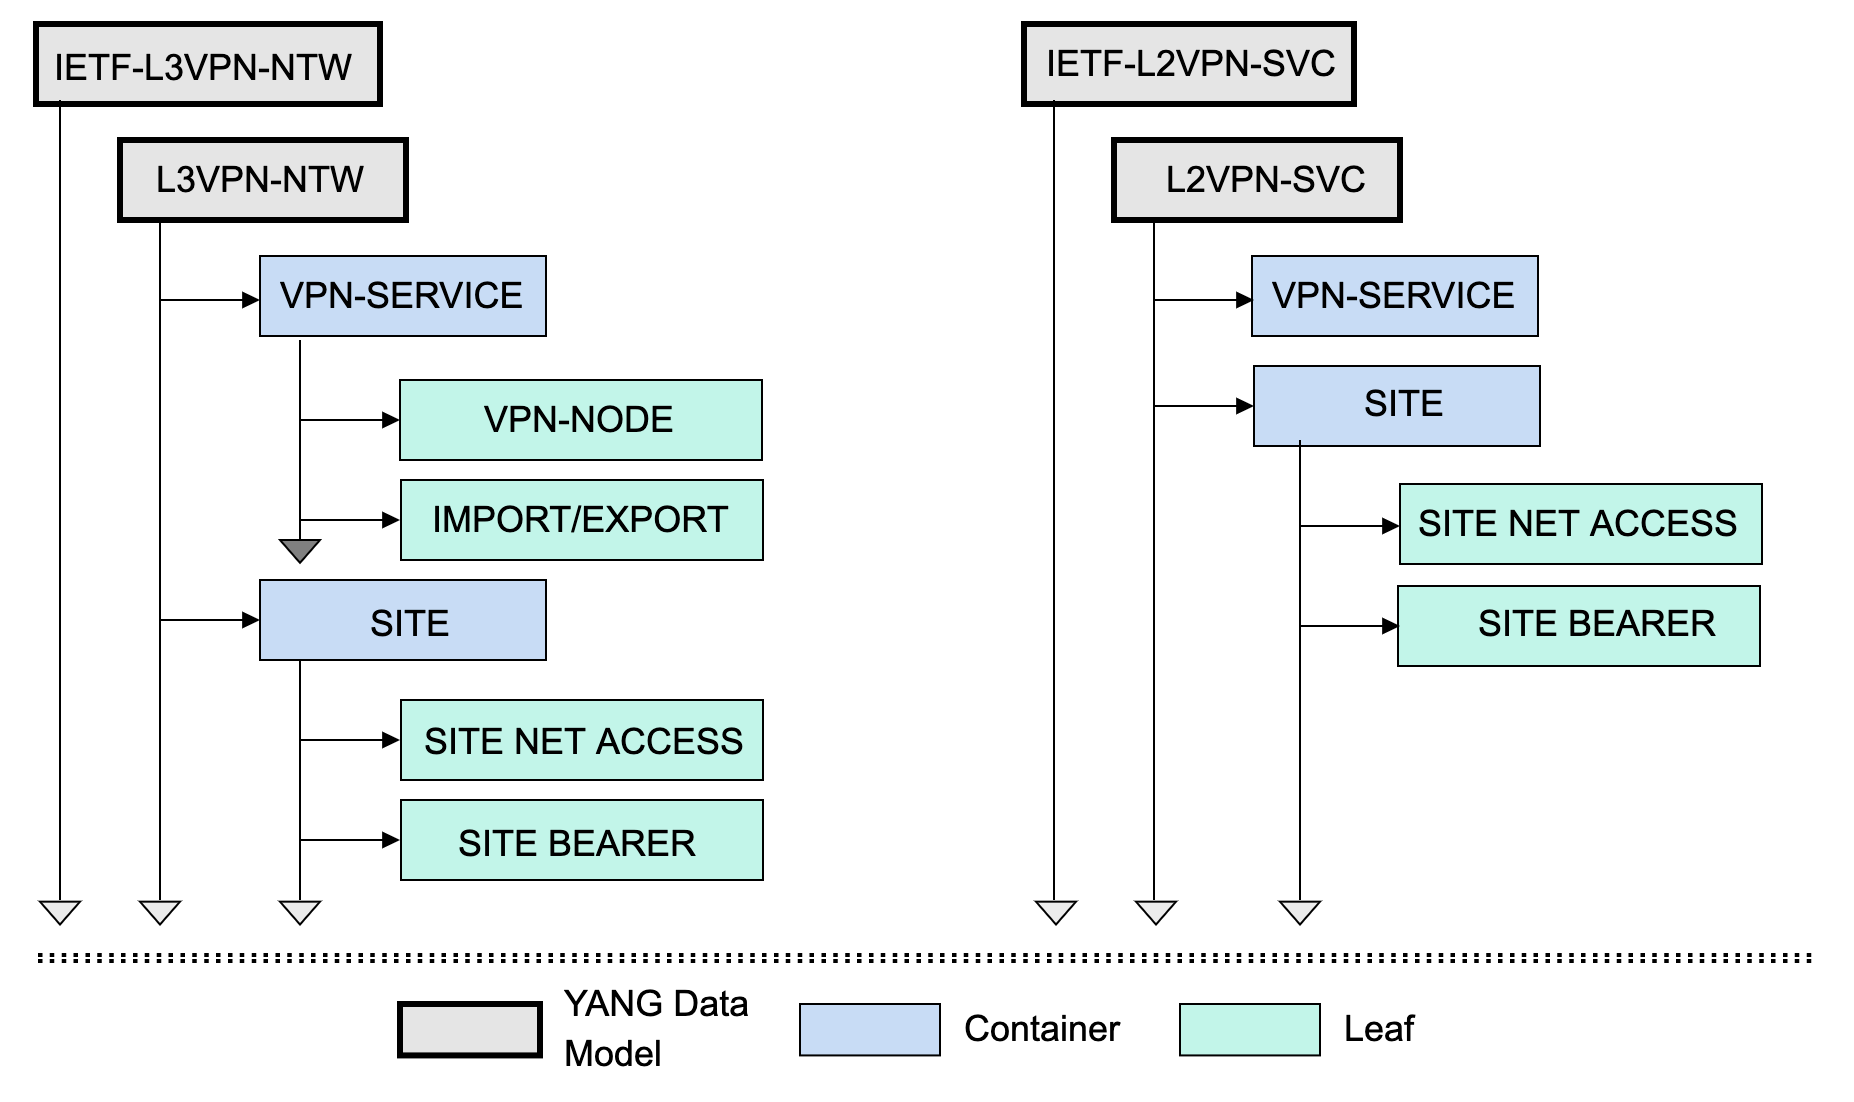
\includegraphics[width=\linewidth]{figs/diagram-10.png}
	\caption{L2NM and L3 Data models structures. The hierarchy represents a container in the YANG model. The  lines represents cross references between the containers.}
	\label{FIG:l3nm} 
\end{figure}

\subsubsection{L2VPN Service Model (L2SM)}
\label{section:l2nm}

Similarly, the IETF has standardized YANG models for the L3VPNs; there is already a standard for the L2 services. The model is named L2SM \cite{wen2018yang}. 

The L2SM is a customer-centric model; It has two main sets of parameters, the VPN Service and the site information. The \cref{FIG:l3nm} depicts the main components of the L3NM and the L2SM as a tree structure. The VPN service contains all the technological parameters of the services that are going to be deployed, for example, service type or service topology. The ``site'' includes all the customer information, like the ``customer-location'' and the access parameters between the Customer-Edge (CE) and the Provider-Edge (PE).

This model lacks some specific network parameters; those need to be stored or derived by the network controller to deploy the network device's configuration. For futures implementations, additional work to complement the current standard can be proposed.  

%\subsubsection{Network Topology}
%\label{subsection:IPtopo}

%The traditional SDN architecture relies on providing different levels of abstraction for each control layer. Therefore, the needs in terms of topology and knowledge of the service provider network differ among components. 

%Network topology is an abstract representation of the physical nodes, links and network interconnections. It is crucial to get and graphically represent network information, such as:
%\begin{itemize}
%    \item Structure (Connectivity and Paths)
%    \item Performance (Available bandwidth per link)
%    \item Availability of physical and logical resources
%\end{itemize}

%Currently, the topology representations are limited to the scope of each of the network vendors i.e., each NMS has its particular/proprietary network view. Sometimes Dummy devices from a third party can be included to simulate the interconnection of the networks. However, nowadays obtain a unified view of the entire IP network is not possible.

%As part of the I2RS working group on the IETF defined a base model for an initial network topology representation has been defined. The model includes nodes and links. As a complementary work, several augmentations have been done over this base to cover the L2, L3, and TE functionalities.

%In this implementation, the topology models used to retrieve the IP network are: 
%\begin{itemize}
%\item IETF Network (RFC8345): Includes the Network, Node and Link concepts.
%\item IETF Network Topology (RFC8346): Includes Termination-Points inside the Nodes and IP specific parameters such as addressing information.
%\end{itemize}

\section{SDN Architecture}
\label{section:arq}
\begin{figure*}[htp]
	\centering
	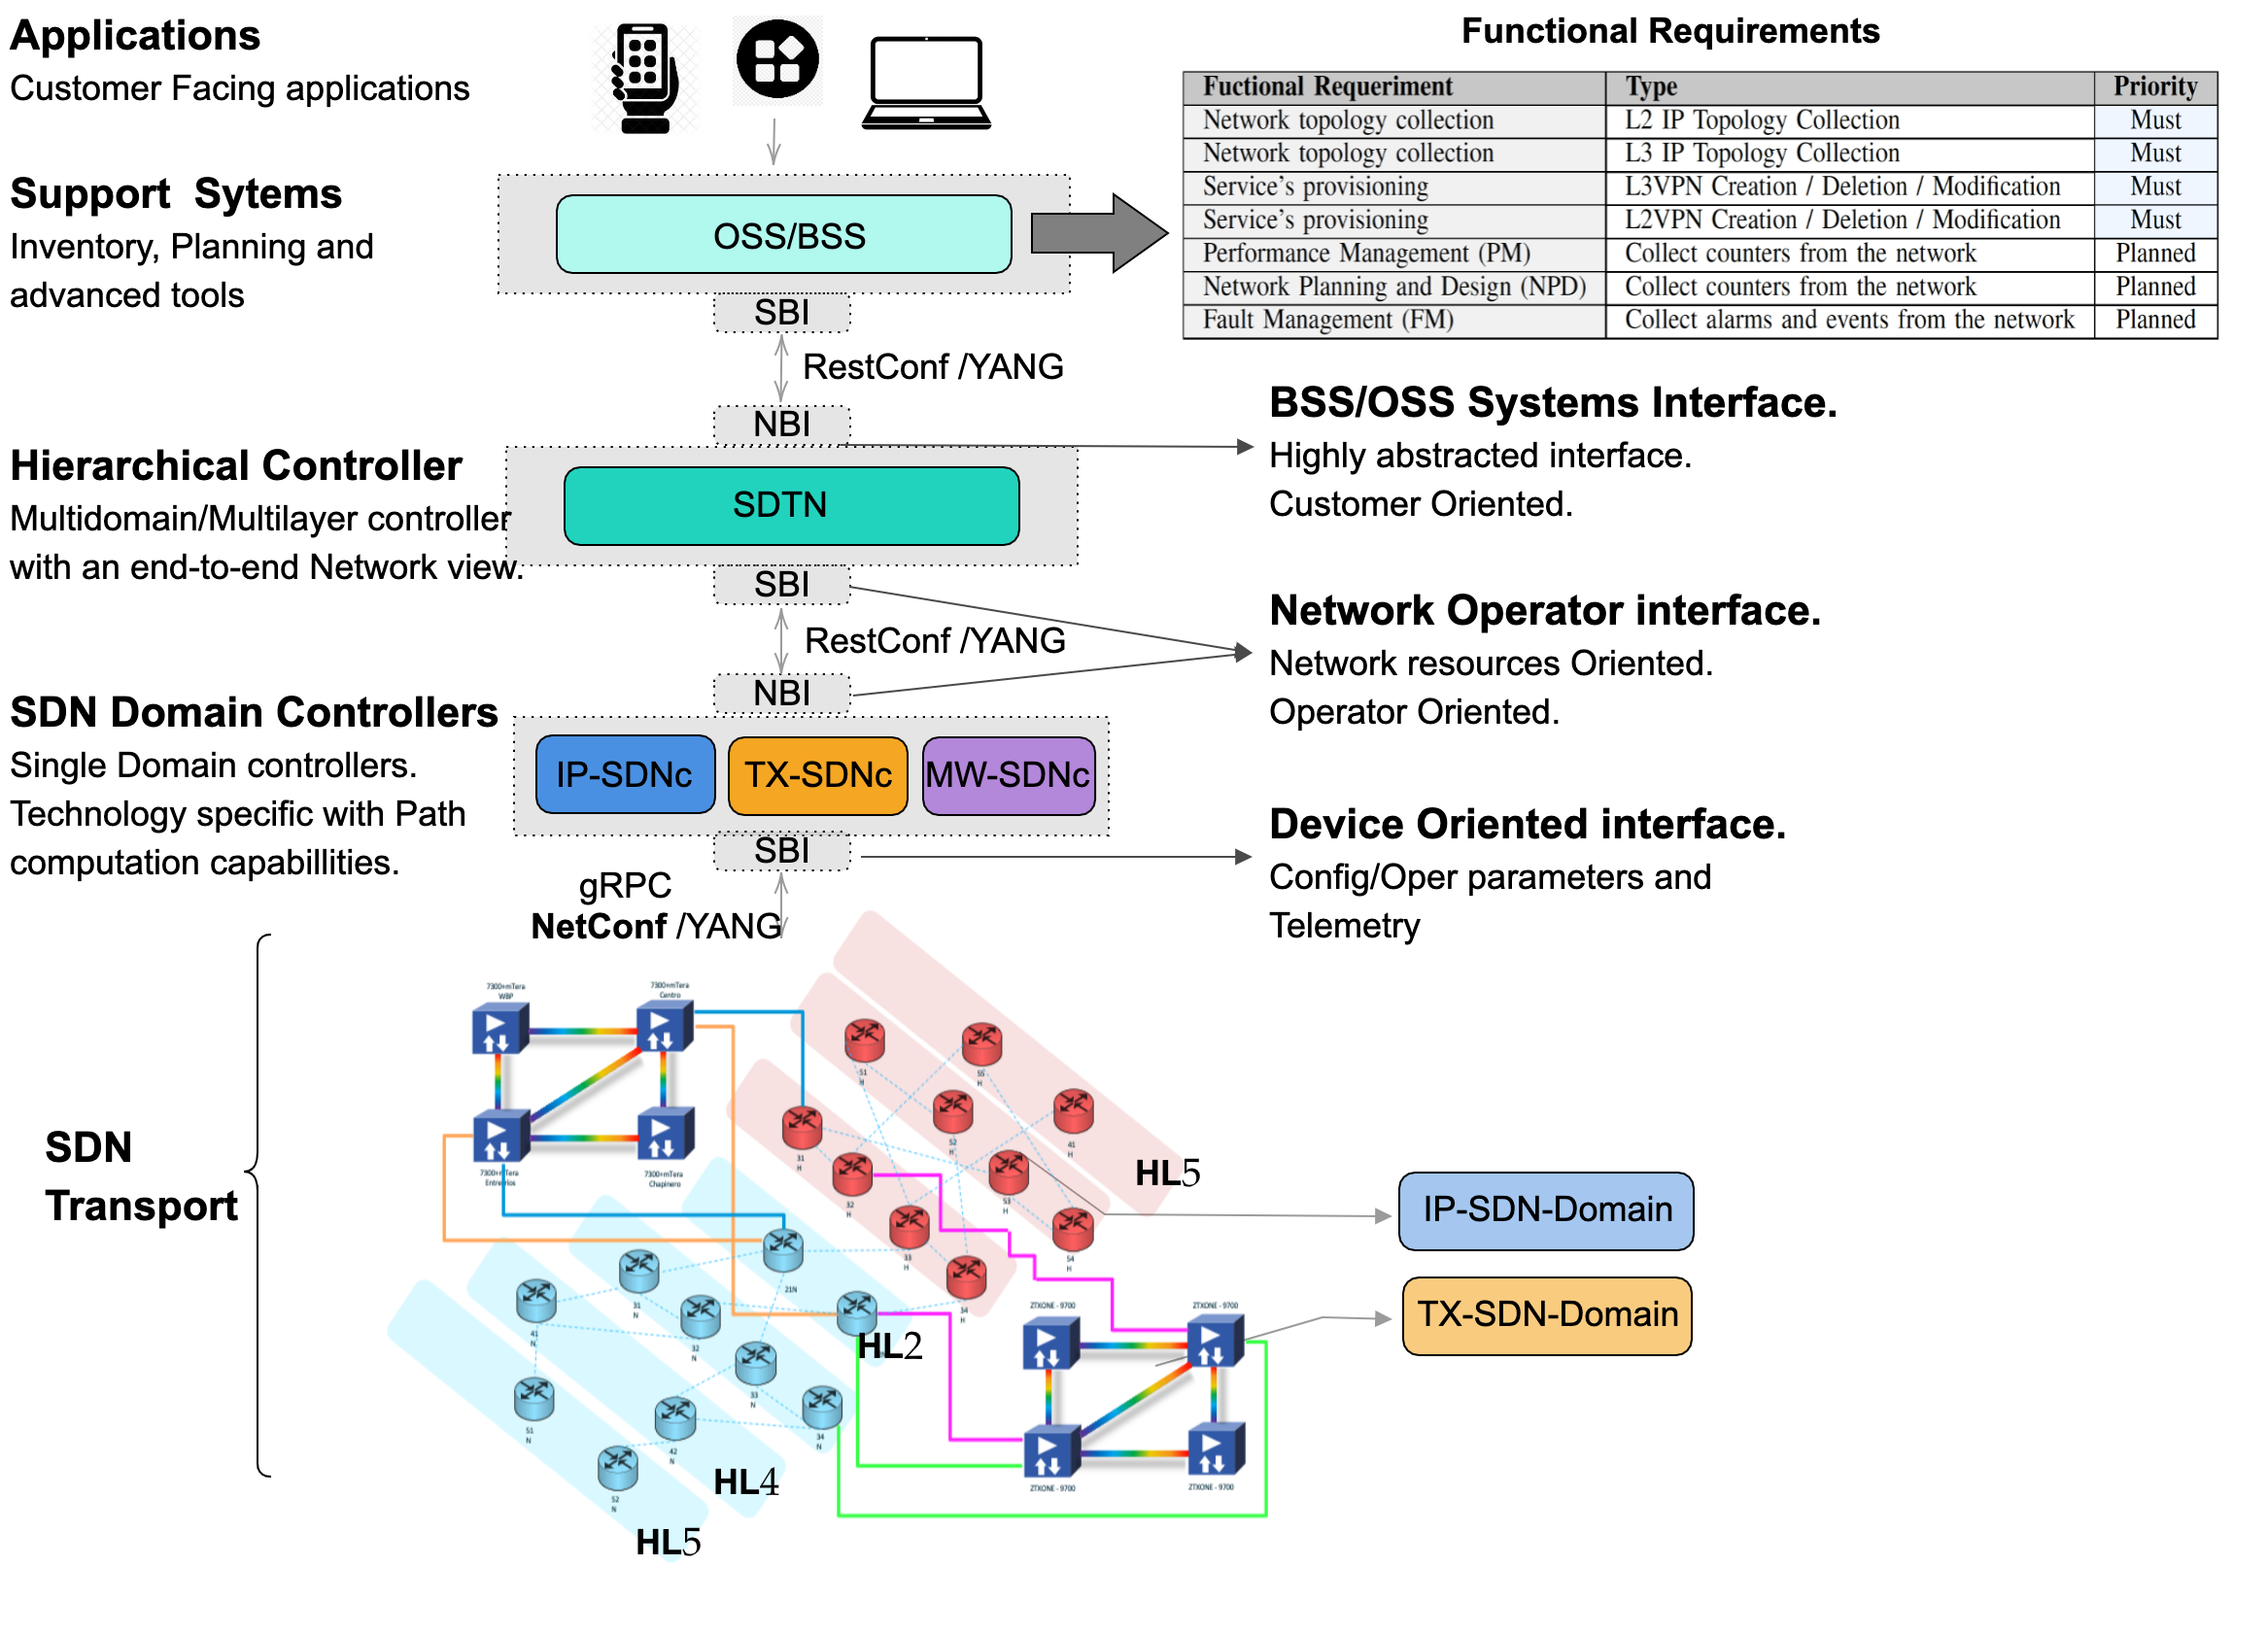
\includegraphics[width=\linewidth]{figs/diagram-1.png}
	\caption{i\uppercase{FUSION}\cite{contreras2019ifusion} architecture has two control layers. The first one having the SDTN controller with the end-to-end view of the network. Second control layer includes the SDN Domain controllers. Those controllers interact with the network devices (Fusion Network). The set of use cases Tested in the POC are listed.}
	\label{FIG:1}
\end{figure*}

%i\uppercase{FUSION} is a reference model architecture defined to reinforce the network automation and programmability in a service provider environment. i\uppercase{FUSION} establishes a clear separation between network and service layers.  The i\uppercase{FUSION} main principles include the use of:

i\uppercase{FUSION} is a reference model architecture defined by Telefonica to reinforce the network automation and programmability in a service provider environment. i\uppercase{FUSION} is hierarchical, with specific domain controllers per technological domain (IP/MPLS, microwave, optical)
and a hierarchical controller to provide real-time control of multi-layer and multi-domain transport network resources. The i\uppercase{FUSION} main principles include the use of: (1) Standard interfaces based on \uppercase{RESTconf/YANG} \cite{bierman2017restconf} for the communication between controllers and \uppercase{NETCONF/YANG} \cite{enns2011network} to configure the network elements; (2) YANG data models based on latest developments in the standards-development organizations (SDOs): \uppercase{IETF}, \uppercase{ONF} and OpenConfig.


The main elements of the SDN i\uppercase{FUSION} architecture are the following:

\begin{itemize}
\item \textbf{SDN Domain}: It is a set of network elements under the supervision of the same SDN Controller. There are several possible levels in the decoupling of control and data planes. The preferred level of decoupling depends on the network technology. For example, network element runs the distributed protocols (e.g. IS-IS TE, RSVP-TE) in MPLS, and the controller only needs to configure it.

%\item \textbf{SDN Transport}: It is the whole network controlled by following SDN principles. It is divided into SDN Domains for technology/scalability/administrative principles. A SDN Transport Controller (also referred as SDN Orchestrator), will take care of stitching the different domains/layers/technologies.

\item \textbf{SDN Domain Controller (SDNc)}: This element is in charge of a set of network elements. It has standard southbound interfaces that depend on the technology, but not in the equipment vendor, to communicate with the network elements. It also has a northbound interface to communicate with the \replaced{SDTN Controller}{SDTN Orchestrator}.\added{For some use cases, like performance management, the authors initially identified the necessity to connect the OSS layer with the SDNc directly.}

\item \textbf{Software Defined Transport Network (SDTN) Controller}: In case several SDN Domains are needed, the \replaced{SDTN Controller}{SDN Transport Controller (SDTN}) is in charge of providing\added{/composing} services through several domains. 

%\item \textbf{Southbound Interface}: It is the interface, based on a standard, between the SDN Domain Controller and the Network Element. Not only the communication protocol needs to be standard, but also the data model used.

%\item \textbf{Northbound Interface}: If is the interface, based on a standard, between the SDN Domain Controller and the OSSs and SDN Transport.
\end{itemize}

The i\uppercase{FUSION} architecture was designed as a hierarchical model where a dedicated SDN Domain controller controls each network segment. Due to its complexity, the transport network is divided into three main technology domains: IP, Optical for transmission, and Microwave.  The proposed architecture can be shown in terms of components and relationships among them, as depicted in \cref{FIG:1}. 

The SDTN Controller is responsible to orchestrate the respective SDNcs within the transport segment (IP, Optical and MW) through the Domain Controllers'~NBI, providing an end-to-end transport network vision. The SDTN Controller aggregates demands from the management and services layer exposing a unified NBI which should provide resource configuration abstraction and technology agnostic service definition. 

%The SDTN entails the following functions: 
%\begin{enumerate}
%    \item End-to-end service binding and mapping.
%    \item End-to-end transport service abstraction.
%    \item End-to-end resource/topology discovery and composition.
%    \item End-to-end resource visualization.
%\end{enumerate}

%The SDN-Cs, on the other hand, are responsible of all the devices in the domain. Each SDN-C unifies the device configuration interface and provides vendor-agnostic network configuration, monitoring and resource discovery. Besides, the SDN-C exposes high-level network services abstraction to OSS and BSS layers through its NBI. Therefore, the abstraction of device-specific configuration from network service definition is one of the main features that the SDN-C implements. Moreover, the SDN-C entails the function of Path Computation Element (PCE) to manage and optimize traffic engineering (TE) in the domain.

\subsection {IP Domain}
\label{section:ip}
Traditionally IP networks are deployed following a regional model mixing equipment from different vendors. The IP boxes are interoperable at both data and control plane levels (e.g., routing protocols such as IS-IS, OSPF, or BGP). Due to scalability and resiliency reasons, the IP administrators divide the whole network into IP domains, so the routing and control protocols are the same in an administrative area.

The goal SDN solution for the IP segment is composed of a single IP \replaced{SDNc}{SDN controller}, whose goal is to configure all the IP network elements. The target SBI for vendor-agnostic device configuration shall be compliant with NETCONF standard protocol. \added{OpenConfig started as a collaborative work between Google, some vendors and Service Providers, and now it is an industrial reference for device-specific configuration purposes. The philosophy behind OpenConfig is to add functionality to the device models based on the operator’s needs to avoid complex models which can not be implemented in real networks.} Due to its maturity level, the set of device configuration data models are the ones defined used in i\uppercase{FUSION} are OpenConfig.
%The IP SDN-C shall perform TE and PCE tasks. With that purpose, some standard and mature control protocols such PCEP and BGP-LS for MPLS networks, shall be implemented to complete the definition of the SBI. As a result, 
It is expected that the IP \replaced{SDNc}{SDN controller} will assume the control/management of:
\begin{itemize}
\item Device configuration of interfaces (VLANs) and routing protocols (BGP, ISIS, …)
\item Traffic Engineering of MPLS tunnels (LSPs). 
\item Overlay networks services (L2/L3 VPNs) device configuration (VRFs,\dots)
\end{itemize}

The IP SDNc will be the main entry point to the network elements, to avoid overloading the elements with external requests and providing a  full and coherent network view. The NBI of the controller in i\uppercase{FUSION} follows IETF YANG models and they are implemented on RESTCONF with JSON encoding. \added{The IETF YANG for the NBI  was done based on the support of the supplier to the models. The IETF adoption is wider than any other alternative for the NBI.}

%The NBI shall provide to higher entities within the SDN hierarchy:
%\begin{itemize}
%\item Device inventory information.
%\item A layered topology view (L2/L3, MPLS) of its controlled network entities.
%\item LSPs provisioning and PCE.
%\item Device abstraction for network services towards the SDTN, i.e., for overlay services VPNs (L2, L3)
%\item Network state and performance monitoring information of the IP domain. 
%\end{itemize}

\subsection{Optical domain}
\label{section:dwdm}
Optical transport networks from different system vendors are deployed on a regional basis, either for technology redundancy, due to different optical performance requirements (metro vs. long-haul), or simply for commercial reasons. 

Without line-side interoperability of the different optical transceivers and Reconfigurable Optical Add-Drop Multiplexers (ROADMs), there is not a competitive advantage on a uniform configuration interface of the optical devices, since they cannot neither be mixed in a multi-vendor scenario, due to the fact that both line systems and transceivers must be from the same vendor.

With this in mind, in the short term, Optical SDNc are expected to provide network programmability and interoperability towards upper layers (multi-layer) and between vendors (multi-domain, multi-vendor) through the support of standard NBIs (i.e. coordination will be provided by upper layer hierarchical SDTN \added{Controller}). This short term approach will enable the setup and tear down of connections in optical channels (OCh and ODU layers), the discovery of the network resources to compose a layered uniform view based on the OTN hierarchy, and the monitoring of the optical network in a vendor agnostic fashion thanks to the utilization of ONF Transport API (T-API) 2.1 \cite{lopez2016transport}, having been experimented in several proof of concepts \cite{mayoral2016first}. Please note, that in this transport domain, T-API + RESTCONF is also proposed to be the NBI of the hierarchical SDTN Controller towards Service B/OSS layers.

%The Hybrid SDN architecture proposed is compatible with a legacy control scenario where a distributed GMPLS control plane has already been deployed. GMPLS control plane can be centrally managed by a SDN domain controller by well-know and mature control protocols, such as PCEP, OSPF and/or BGP-LS already supported in GMPLS devices, benefiting the gradual introduction of SDN. However, current NMS solutions shall evolve to, or co-exist with, the SDN Controller model, enabling network programmability through its NBIs while keeping the current offered features for network creation, resources discovery and monitoring and service creation for L0/L1 layers. Standardization efforts targeting the definition of standard NBIs that can facilitate multi-vendor interoperability (by maintaining administrative domains for each vendor) such as ONF Transport API (T-API) \cite{lopez2016transport} and IETF models \cite{rfc8299} are the more promising definitions to implement such capabilities by abstracting the specific configuration of current distributed control planes embedded in Automatic Switched Optical Network (ASON) architectures. 
%i\uppercase{FUSION} relays on ONF Transport API 2.1 as as the reference NBI for the SDN implementation in the optical transport segment, having been experimented in several proof of concepts \cite{mayoral2016first}. 

In the medium and long term, the direct programmability of the components can have interest in Point-To-Point, Metro and Regional scenarios, where disaggregation of optical transceivers and line side components can play an important role. In this line, OpenROADM \cite{oda2016learning} and OpenConfig projects have already defined device configuration models for transponders and open line systems. 
%Telefonica is approaching this transformation of the optical control in two phases:

%\begin{enumerate}
%    \item \textbf{Partial disaggregation}: As a medium term objective, where the target is to define a standard interface based on NETCONF/YANG, which allows of the Optical SDN-C to manage third-party terminal devices (i.e., transponders) that can transmit over the vendor line system.
    
%    \item \textbf{Full disaggregation}: The long term objective is the open management of the line system, i.e., the defragmentation of the optical transport network in vendor islands by the adoption of a common standardized interface for open line systems (multi-vendor) to be managed by a single optical SDN-C.
%\end{enumerate}
%In this section the reference standard model use for the control/management of networks based on WDM/OTN technologies is described. 
%The proposed solution for the Optical SDN-C's NBI is based on ONF T-API information models \cite{mayoral2016first}.  NBI message transportation is performed using the RESTCONF protocol. Please note, that in this transport domain, the same solution (T-API + RESTCONF) is also proposed to be the NBI of the hierarchical SDTN Controller towards Service B/OSS layers.

%\subsubsection{Provisioning}
%
%\begin{figure*}
%	\centering
%		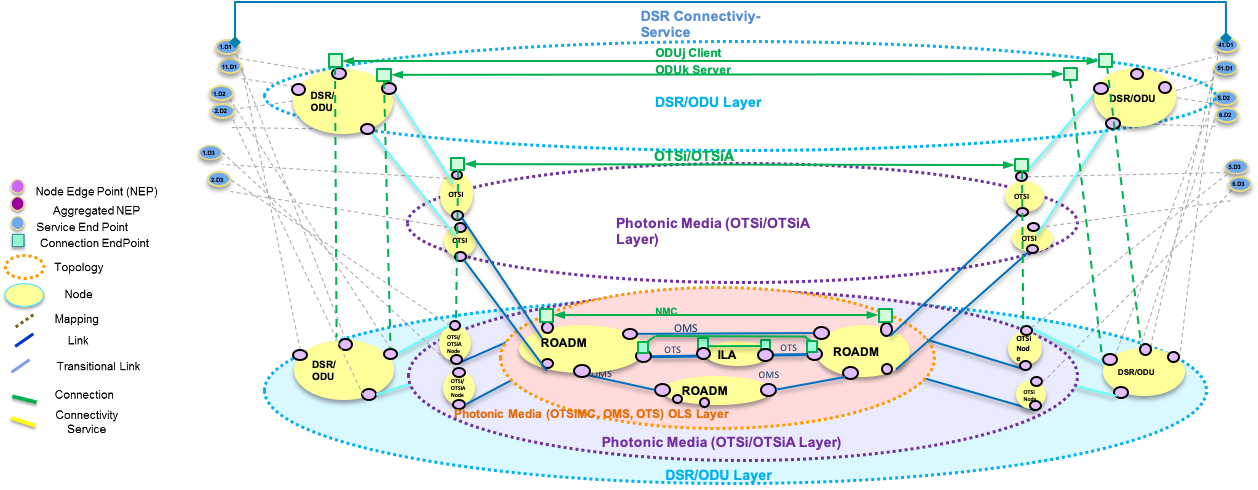
\includegraphics[scale=0.75]{figs/ONF-T-API.png}
%	\caption{Multi-layer topology and connectivity models based on ONF T-API}
%	\label{FIG:ONF-T-API}
%\end{figure*}

%The connectivity provisioning into the WDM/OTN optical layers is strictly related with the model proposed. \ref{FIG:ONF-T-API} represents the optical network topology arrangement proposed in the previous figure and the multi-layer hierarchical connectivity modelling which is being detailed in this section.

%The connectivity model introduces to central concepts. On one hand, the tapi-connectivity:connectivity-service  object models "intended" solicited by the T-API client layer, to be deployed into the network. On the other hand, the tapi-connectivity:connection objects represents the actual adjacencies between logical interfaces created by configuring the network, in brief the connectivity configurations in the network. 

%The network model is multi-layer so it is needed to establish multi-layer relationships into the model. These relationships are construct by the relationship between Logical Termination Points (LTPs) which in T-API are modelled as two different objects: the Node-Edge-Points (NEPs) which represents the resources available at a give layer LTP to provide connections, and the \textbf{Connection-End-Points (CEPs)} which consumes part of all of the NEPs exposed resources to create the connections between different points of the network. In our proposed reference implementation, we distinguish between two different level of connections:

%\begin{itemize}
%    \item \textbf{Cross-Connections (XC)}: defined as a connection between Connection-End-Points of the same layer within a Forwarding-Domain (represented as a\\ \texttt{tapi-topology:node} object). 
%    \item \textbf{Top Connections}: are defined as end-to-end connections between CEPs within the same layer which may span multiple Forwarding-Domains. Top connections are composed by zero or more XCs which belong to the same layer of the Top Connection.
%\end{itemize}

%Then, the multi-layer relationships are construct by stacking CEPs over NEPs and providing the upper layer resources representations by the dynamic creation of new NEPs, e.g., an OTSi connection, when created and operational, it provides the ODU upper layer resources in the form of NEPs which in turn can be consumed to create ODU connections which will provide the DSR layer resources.

%\subsubsection{Topology}
%\label{subsection:OPTopo}

%The topology model should provide the explicit multi-layer topology representation of the L2-L0 network including OTS, OMS, MC, OTSIMC, OTSi/OTSiA, ODU, DSR layers. The network logical abstraction collapses all network layers (DSR, ODU, OTSi/OTSiA and Photonic Media (OTSiMC, MC, OMS, OTS)) which are represented explicitly into a single topology (T0 – Multi-layer topology), modelled as a \texttt{tapi-topology:topology} object within the: \\
%\texttt{tapi-topology:topology-context/... \\
%... tapi-topology:nw-topology-service} and \\ \texttt{tapi-topology:topology-context/topology}. 

%The T0 – Multi-layer topology MUST include:

%\paragraph{DSR/ODU Layers:}
%DSR/ODU forwarding domains represented as multi-layer and multi-rate \texttt{tapi-topology:node}, allowing the representation of the internal mapping between DSR and ODU NEPs (multi-layer) and the multiplexing/de-multiplexing across different ODU rates (multi-rate). 

%The DSR/ODU layer network MUST be represented explicitly at the lowest partitioning level, i.e., each DSR/ODU forwarding domain MUST be represented as a single tapi-topology:node. The following network components included within the category of ODU forwarding domain are:

%\begin{itemize}
%    \item Transponders.
%    \item Muxponders.
%    \item OTN switching nodes connecting client and line %boards.
%\end{itemize}

%\paragraph{OTSi/Photonic Media layers:}
%The OTSi layer represents the optical side of the optical terminals (transponders/muxponders). This layer consists of nodes representing the mapping and multiplexing of OTSi signals. It consists of nodes including OTSi client endpoints representing the Trail Termination Points (TTPs) of the OTSi connections and OTSi/OMS endpoints representing the physical connectivity with ROADM/FOADM add/drop ports.

%DSR/ODU and OTSi layers may be collapsed into a single multi-layer node or split into two logical nodes representations by using the Transitional links concept to represent the potential layer transitions between ODU and OTSi.

%\paragraph{Photonic-Media layer:}
%The Photonic-Media layer models the Optical Line Protection  (OLP) components, the Reconfigurable/Fixed Optical Add Drop Multiplexers (ROADM/FOADM) and In-Line Amplifiers (ILAs) network elements. Moreover, all the lowest photonic connectivity is represented as PHOTONIC\_MEDIA \texttt{tapi-topology:link} objects collapsing OTS/OMS layers and allowing placing specific monitoring OAM functions of these layers. These forwarding domains SHALL expose the capability of create Media Channel connection and connectivity services between its endpoints.

%\begin{figure}
%	\centering
%		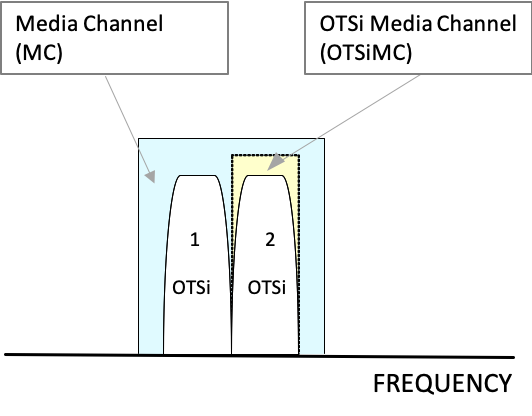
\includegraphics[scale=0.75]{figs/Media_channel.png}
%	\caption{Media-channel entities relationship}
%	\label{FIG:Media_channel}
%\end{figure}

%Moreover, the Media Channel layer the available resources for the reservation of  spectrum resources for a given OTSi channel. The concatenated reserved portion of the along a route is represented as a Media-Channel (MC) construct, and by the OTSiMC construct which represents the actual portion of the spectrum occupied by the signal (MC spectrum must be wider than the OTSiMC). These modelling concepts are critical for the realization of the Open Line System concept introduced by the partially disaggregation of the optical networks. See \ref{FIG:Media_channel} graphical representation for more clarity.

\subsection{Integration of SDTN \added{Controller} in the overall operator’s systems architecture}
\label{section:sdtn}
One of the main reasons for deploying an SDTN Controller is service automation. It facilitates that manual services and network configurations become automated and available through its NBIs, enabling the network automation progressively. As the main design principle, the abstraction level provided by the SDTN \added{Controller} can be different based on the needs of consumers. Thus, the information exported through the NBI towards OSS and other platforms will cover several functional areas with several levels of abstraction: (1) network topology, (2) service provisioning, (3) performance management, (4) network planning and design, and (5) fault management. 
%\begin{itemize}
%    \item \textbf{Network topology}: An hierarchical topology view of the network % resources, based on the OSI layers.
%    \item \textbf{Service’s provisioning}: The available set of network services % to different clients.
%    \item \textbf{Performance Management (PM)}.
%    \item \textbf{Network Planning and Design (NPD)}.
%    \item \textbf{Fault Management (FM)}.
%\end{itemize}

% Please add the following required packages to your document preamble:
% \usepackage[table,xcdraw]{xcolor}
% If you use beamer only pass "xcolor=table" option, i.e. \documentclass[xcolor=table]{beamer}


%\begin{table}[]
%\caption{Set of use cases Tested in the POC}
%\label{TAB:use_cases}
%\begin{adjustbox}{width=0.5\textwidth}
%\begin{tabular}{|
%>{\columncolor[HTML]{EFEFEF}}l |l|c|}
%\hline
%\cellcolor[HTML]{C0C0C0}\textbf{Fuctional Requeriment} & \cellcolor[HTML]{C0C0C0}\textbf{Type}      & \multicolumn{1}{l|}{\cellcolor[HTML]{C0C0C0}\textbf{Priority}} \\ \hline
%Network topology collection                            & L2 IP Topology Collection                  & \cellcolor[HTML]{ECF4FF}Must                                   \\ \hline
%Network topology collection                            & L3 IP Topology Collection                  & \cellcolor[HTML]{ECF4FF}Must                                   \\ \hline
%Service’s provisioning                                 & L3VPN Creation / Deletion / Modification   & \cellcolor[HTML]{ECF4FF}Must                                   \\ \hline
%Service’s provisioning                                 & L2VPN Creation / Deletion / Modification   & \cellcolor[HTML]{ECF4FF}Must                                   \\ \hline
%Performance Management (PM)                            & Collect counters from the network          & Planned                                                        \\ \hline
%Network Planning and Design (NPD)                      & Collect counters from the network          & Planned                                                        \\ %\hline
%Fault Management (FM)                                  & Collect alarms and events from the network & Planned                                                      \\ %\hline
%\end{tabular}
%\end{adjustbox}
%\end{table}

Network topology and service provisioning are tested in this paper, the full set of use cases tested as described in the \cref{FIG:1}. Progressively, the SDTN \added{Controller} will include the rest of the functionalities (marked as planned). On its SBI, the SDTN \added{Controller} will integrate with the domain controllers. Each SDNc shall expose vendor-agnostic network-level programmability and resource discovery functionalities. So the SDTN \added{Controller} will be able to perform the correct data integration and functionalities exposure.

%On its SBI, the SDTN will integrate with the domain controllers; Each Transport SDN-C shall expose vendor-agnostic network-level programmability and resource discovery functionalities. So the SDTN will be able to perform the correct data integration and exposure.

%On the SBI of the SDTN, each technology Transport SDN-C shall expose vendor-agnostic network level programmability and resource discovery functionalities. The SDTN's SBI is intended, but not limited, to provide access to device’s configuration data, to expose per-OSI layer topology and network inventory information, and to offer active monitoring of device configuration changes and network state data (i.e., traffic statistics). Alarm and device inventory information for FM and RIM respectively, is intended to be managed at the SDN-C in a first phase, but its exposure through the SDTN will be evaluated too.


%\section{Network Programmability}
%\label{section:net}

%The network management has lagged behind other technologies quite drastically. In more than 20 years, there has not been radical improvements in the device management area. One of the major advances was related to the usage of SSH instead of TELNET for secure implementations. However, scripts based on EXPECT are the most programmatic way to access the devices in the service providers across the globe.

%This lack of manageability is often better understood when networking is compared with other technologies. For example, hypervisor managers, wireless controllers, IP PBXs, PowerShell, DevOps tools are part of the continous Integration and continous Development (CI/CD) in cloud providers \cite{mittal2017cloud,demchenko2016zerotouch}. Some of these are tightly coupled from a certain vendor, but others are more loosely aligned to allow for multi-platform management, operations, and agility \cite{edelman2018network}.

%To allow the network programmability it is completely necessary to use SDN as the reference for the introduction of network APIs. It must be taken into account that these network APIs are not just related to the service provision automation (provision is a repetitive task and its components can be described in a technological way). The usage of APIs and programmatic interfaces can automate and offer much more than pushing configuration parameters. 

%It can be used to cover all the FCAPs (Fault, Configuration, Accounting and Performance) capacities and Network planning tasks:
%\begin{itemize}
%    \item Network planning tasks if we include APIs to export distributed information such as the RIB, FIB, and TE-Databases.
%    \item Used to deploy close-loop decision systems to take actions based on events reported by the devices.
%    \item Automatically visualize the network relationships between the IP/MPLS and Optical packet transport domain. Creating a common network view. 
%\end{itemize}

%\section{Service Models}
%\label{section:models}

%Due to the network programmability necessities. Protocols and Data models must be selected to allows the interaction between the network controllers and devices. There has been a great interest in using YANG to define these data models. However, this YANG-based set of definitions may include two groups of models. One set used strictly to attack the devices and the ones used to describe services in a portable and technological way (independent of which network operator uses the model). 
%This differentiation between Service and Device Models introduced in early 2018, would allow abstract some information in the control layer. The service models may be used as part of the SDN architecture, describing the data interchanged between the network controllers and between OSS systems and the control Layer \cite{wu2017service}. While the device models described the specific configuration of the network elements. 

%Example of service models definitions used during this implementation are described in \ref{section:IPmodels} for IP and \ref{section:OPTmodels} for Optical.

\subsection{Multi-domain IP L3VPN provisioning}
\label{section:muli-l3nm}

The L3VPNs services are not exclusive of single domain implementations; multi-domain IP L3VPN is a common requirement in the service providers. Multi-domain services include: multiple-AS, multiple-IGPs, or multiple-vendor segmentations. Based on this, a set of interactions with more than one IP SDNc may be required to accomplish the service provision process.

The scope of this work includes two IP domains connected by a common core; The IP domains were part of a different IGP process, so each network has its own IP SDNc. Each of the controllers has implemented the IETF L3NM model described in subsection \ref{section:l3nm} to support the service creation requirements. We have proved the SDTN \added{Controller} as a network orchestrator to create a multi-domain L3VPN, delegating the required provision parameters to each domain controller and after exposing a unified view of it.

\begin{figure}
	\centering
		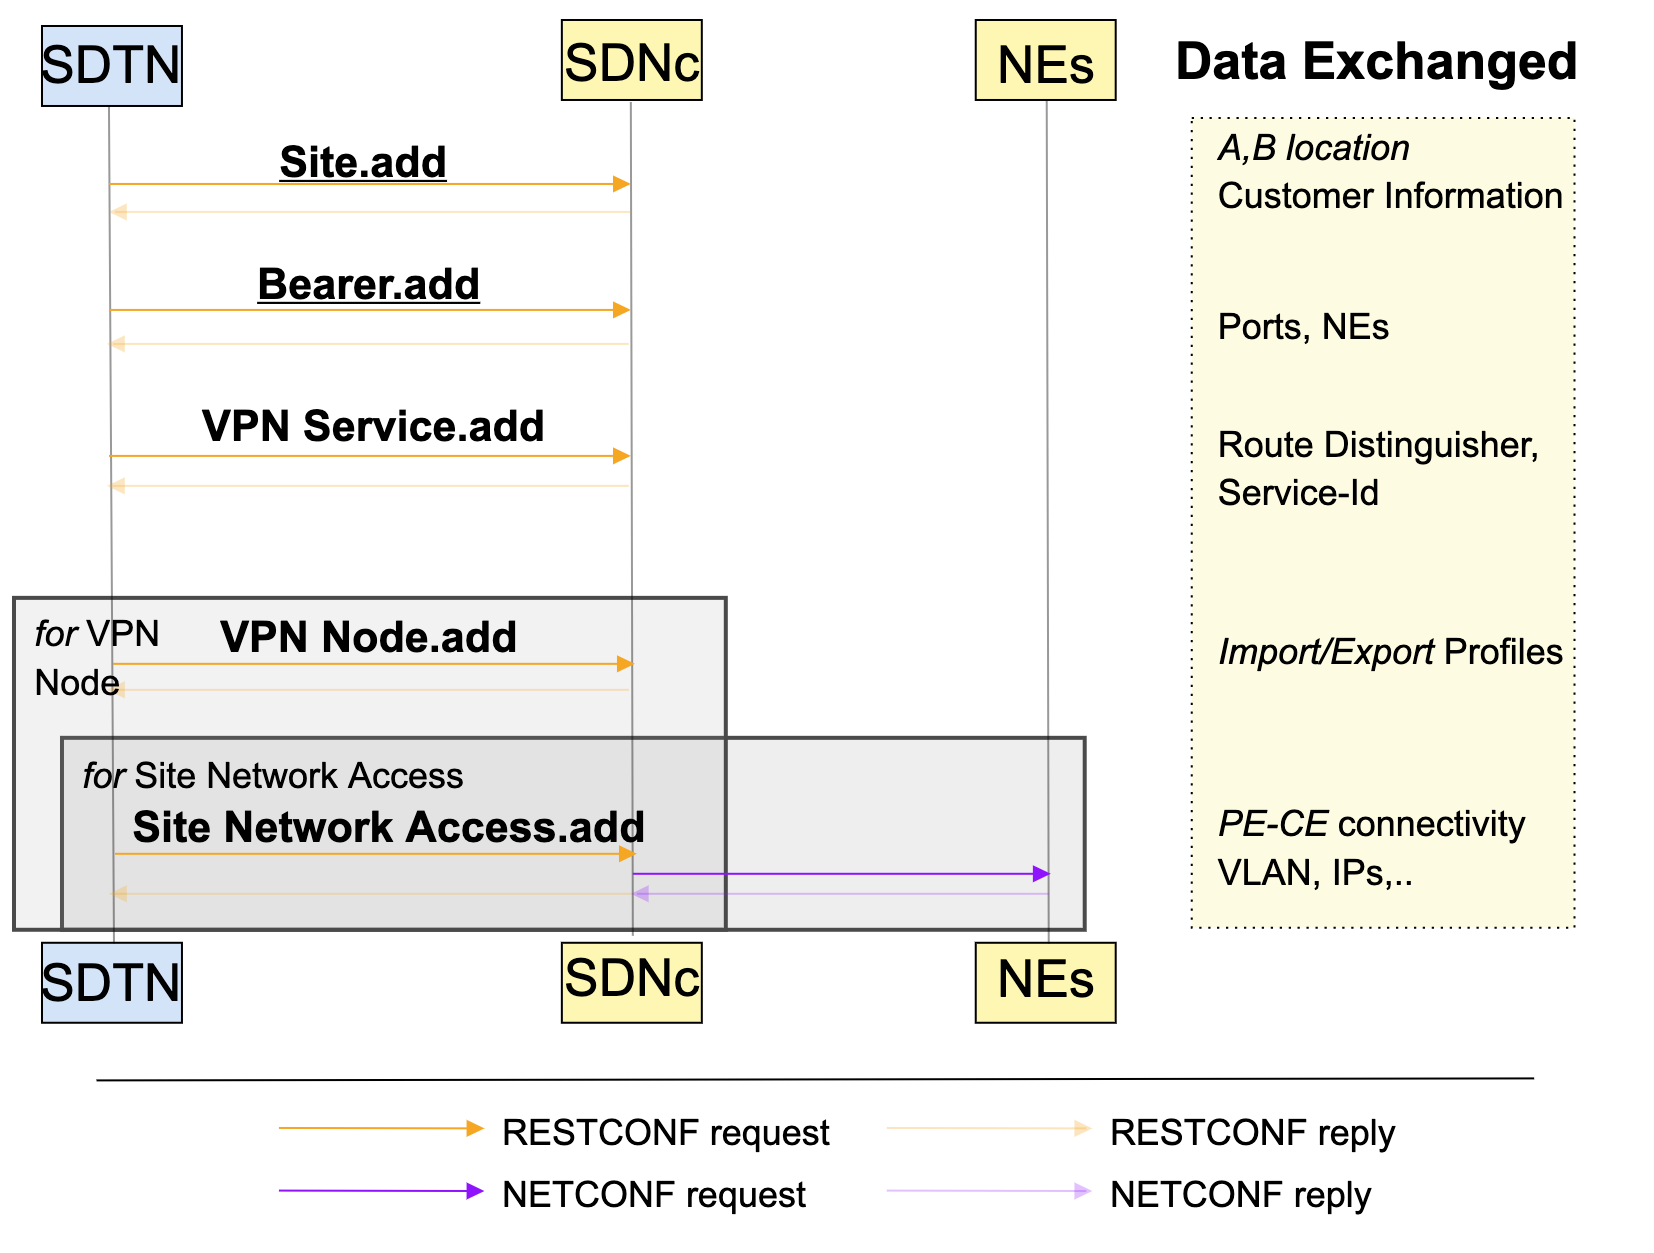
\includegraphics[width=\linewidth]{figs/diagram-9.png}
	\caption{Messages Interchange for IP multi-domain L3VPN service creation.}
	\label{FIG:l3vpn_workflow}
\end{figure}

The parameters delegation done by the SDTN \added{Controller} had the following four steps per domain.
\begin{enumerate}
    \item Create Site: Indicates the place where the services end-points are located. It unclude magement information and service descriptions. 
    \item Create Bearer: Indicates the NE and the Port assigned to the service.
    \item Create VPN-Node: Indicates the VRF deployment and all its attributes on the PE. It includes the import/export policies.
    \item Create Site Network Access: Refers to the CE-PE connectivity attributes. Such as routing protocol exchanged, IP addressing or ethernet encapsulation. 
\end{enumerate}

\Cref{FIG:l3vpn_workflow} depicts the corresponding workflow to create the L3VPN. Each step in the figure matches the sequence previously described. A similar workflow was used for all the RESTCONF operations like Create, Read, Update and Delete. 

%\begin{figure}
%	\centering
%		\includegraphics[width=\linewidth]{figs/multidomain_service_provisioning%_workflow.png}
%	\caption{Workflow for multi-domain service provisioning SDTN-SDN-C}
%	\label{FIG:multidomain_service_provisioning_workflow}
%\end{figure}

%\subsubsection{Multi-layer Topology}

%The multi-layer topology use case is based on the data provided by all the IP and Optical WDM/OTN SDN-Cs. The scope of it, includes the composition of multiple sources and data-formats (i.e IETF context for IP or T-API context for Optical) to create a common view of the network. The models used to create the multi-layer topology were:
%\begin{itemize}
%    \item For the optical domain representation: Topology and Connectivity Service modules. Those models provides information for layers from L0 to L2.
%    \item For the IP/MPLS domain representation: The IETF\\ \texttt{ietf-network:networks} is the basis to expose the network model(nodes and IP Links), and the \\ \texttt{.../node/nt:termination-point}
%    were used to expose the Terminations-points (Ports) of a specific node.
%\end{itemize}
    
%Additionally, a correlation parameter is defined to join the IP and Optical layers. We have denoted this parameter as the \texttt{Plug-id}. This additional definition is needed due to there is no a dynamic protocol or common element between the ONF/IETF standards that would allow their direct correlation. The \texttt{Plug-id} parameters is added in the IETF termination points and in the T-API connectivity services. 

%It is necessary to remark in the T-API model side the \texttt{Plug-id} parameter is a "String" and in the IETF side is "Binary", therefore the SDTN MUST have the ability to traduce the “Binary” value to “String” or vice versa, to be able to make the match in the correlation process considered to be standardized.

%To fill the \texttt{Plug-id} attribute automatically between the layers, it is required that the SDTN performs a process based on meta-heuristic algorithms. In which, the performance data at termination-points level both in the IP and in the Optical layers will be correlated. Clock \& Time must be perfectly synchronized between the Tx/Rx points, bidirectionally. Meta-heuristics must include the geo-location parameter of the nodes as input. However, the design of this process is currently under study and is based on real-time information that can be delivered by the telemetry engines.

%\begin{figure}
%	\centering
%		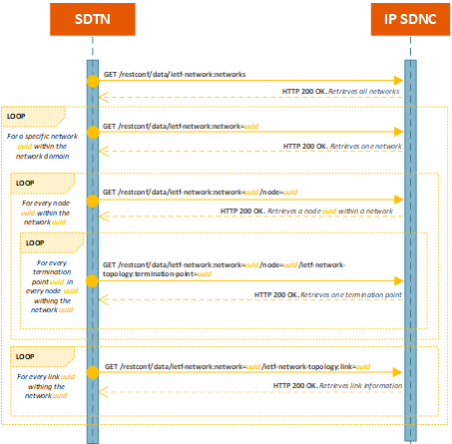
\includegraphics[width=\linewidth]{figs/ip_topology_workflow.png}
%	\caption{Message Interchange for IP Topology Discovery between the SDTN and IP SDN-C}
%	\label{FIG:ip_topology_workflow}
%\end{figure}

%Starting with the Optical Domain, a set of T-API version 2.1 queries were sent in order to build the topology by extracting the list of networks as well as topology details such as nodes, links, connections and service-interface-points available. The query exchange process between is shown in the UML diagram depicted in \ref{FIG:optical_topology_workflow}.  

%\begin{figure}
%	\centering
%		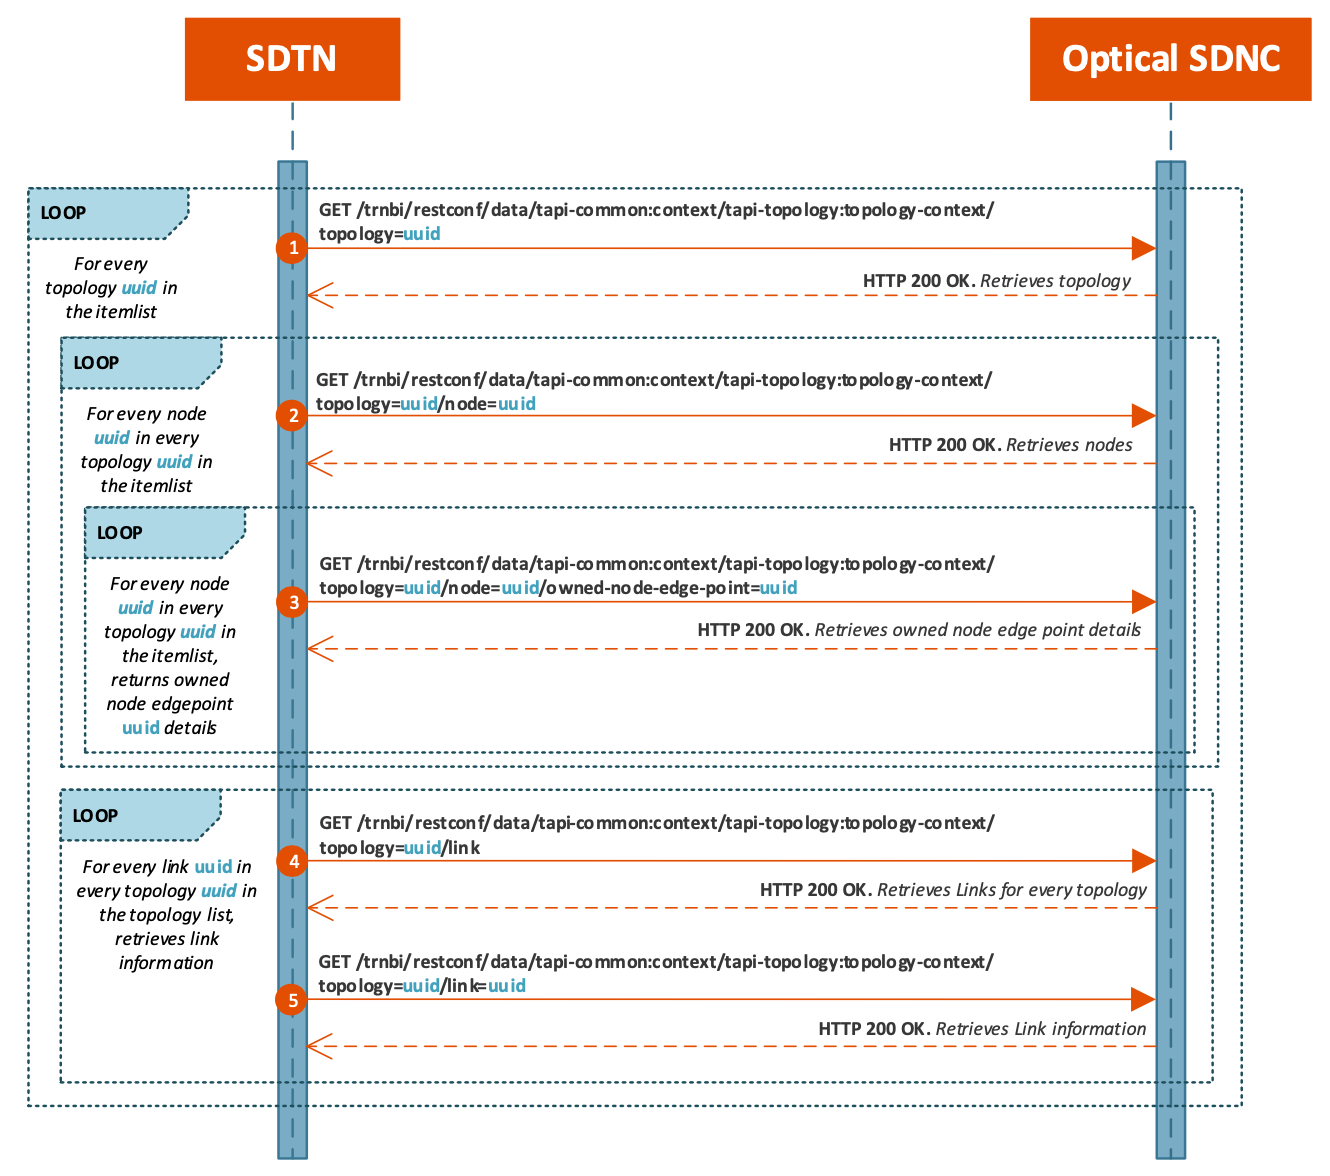
\includegraphics[width=\linewidth]{figs/optical_topology_workflow_2.png}
%	\caption{Messages Interchanged for Optical Topology Discovery between the SDTN and Optical SDN-C}
%	\label{FIG:optical_topology_workflow}
%\end{figure}

%Regarding the IP Domain, to obtain the whole network topology, a query to the controller’s NBI to retrieve the network topologies available for all layers is sent; from here on, the client must perform per-layer queries to get more detailed information such as nodes, termination points of nodes, links, etc. \ref{FIG:ip_topology_workflow} displays the RESTCONF based queries in UML format for the topology retrieval in the IP Domain. 
%At this point, no inter-domain links were retrieved since there is no automatic mechanism supported on the domain controllers to expose information such as TTI (on the Optical Domain), LLDP (on the IP Domain) or \texttt{Plug-id} (for both domains); therefore \texttt{Plug-id} based link discovery was simulated by adding user defined \texttt{Plug-id} values to each port or at least to each domain edge port manually with the use of Python scripting. The inputted plug-id data was automatically detected by the SDTN and the inter-domain links between ports with matching \texttt{Plug-ids} were created, resulting in a complete multi-layer/multi-domain end-to-end topology as seen from the SDTN GUI.

%\begin{figure}
%	\centering
%		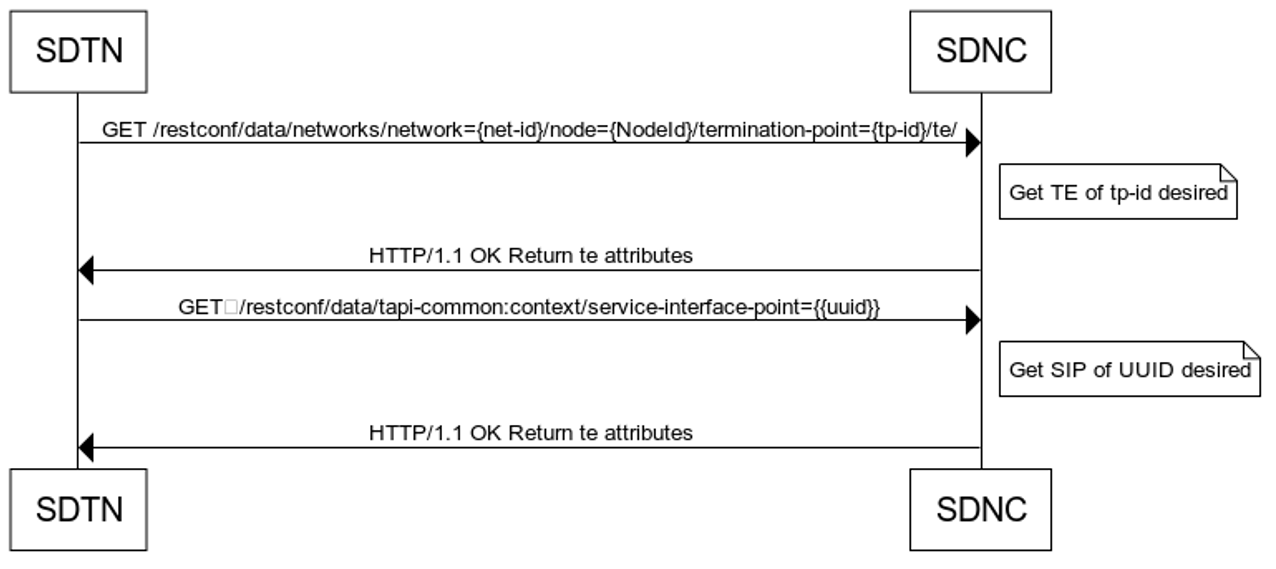
\includegraphics[width=\linewidth]{figs/topology_workflow.png}
%	\caption{Workflow for multi-layer topology SDTN-SDN-C}
%	\label{FIG:topology_workflow}
%\end{figure}

%\begin{figure*}
%	\centering
%		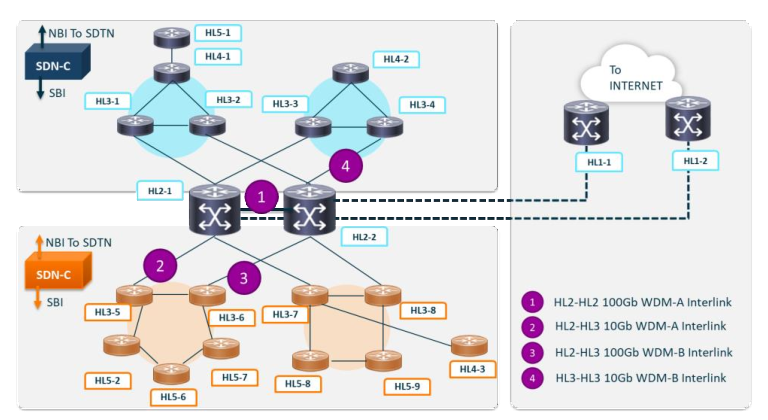
\includegraphics[scale=1]{figs/field_trial_environment_ip.pdf}
%	\caption{Network Plane of the Field Trial Environment for IP/MPLS Testing and Evaluation}
%	\label{FIG:field_trial_ip}
%\end{figure*}

%\begin{figure*}
%	\centering
%		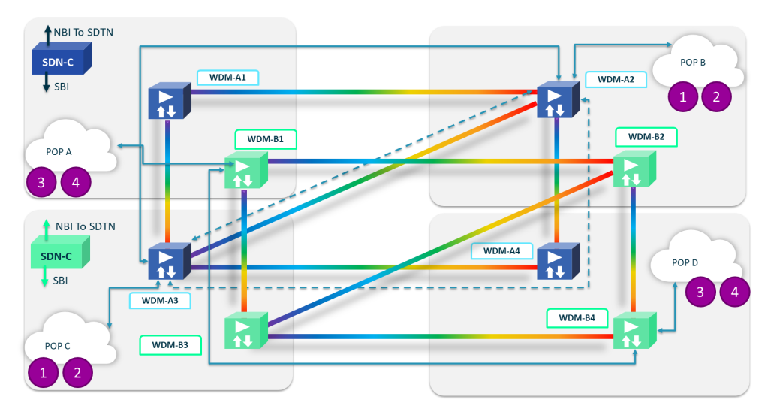
\includegraphics[scale=1]{figs/field_trial_environment_optical.pdf}
%	\caption{Network Plane of the Field Trial Environment for Optical/WDM Testing and Evaluation}
%	\label{FIG:field_trial_optical}
%\end{figure*}

\section{Field Trial Environment for i\uppercase{FUSION} SDTN Demonstration}
\label{section:trial}

In this work, we have deployed the i\uppercase{Fusion} architecture in a Telefonica Colombia field trial environment. The field trial includes not just the i\uppercase{FUSION} SDN control layer (\Cref{sec:contollay}), but also the network elements described in \Cref{sec:netlay}.%, which is a multivendor IP/MPLS network using an underlying optical infrastructure.

\subsection{SDN Control Layer}
\label{sec:contollay}
The SDN control layer architecture was built upon the reference design guidelines described in \Cref{section:arq}. The key elements of the control layer was:
\begin{itemize}
    \item Infinera Trascend Maestro, acting as SDTN controller.
    \item 2 x IP SDNcs one for each IP domain. 
    \item 2 x Optical SDNcs one for each optical domain.
\end{itemize}

SDNcs communicate with NEs via NETCONF/YANG and RESTCONF/YANG with SDTN \added{Controller} using the Data Communication Network (DCN). The optical and IP SDNcs are commercial products from the network element vendors.  

%In other hand, from the Optical perspective, SDN-Cs follow a similar integration. At SBI, OpenROADM + OpenConfig models are used on top of NETconf/YANG protocol. At NBI, a T-API v2.1 implementation is used.  

\subsection{Network Elements}
\label{sec:netlay}
The set-up for this field trial uses a full network with all the Hierarchical Levels (HL) that compose a Service Provider real environment. In our notation and architecture the IP/MPLS-based network is comprised of five (5) HLs with the following responsibilities: 

\begin{itemize}
    \item HL1: Core PE-Routers acts as Toll Gates for the Service Provider's interconnection with other carriers and using eBGP logical structure for publishing public IPv4/IPv6 prefixes. 
    \item HL2: Core P-Router is responsible for the transportation of traffic between main cities and metropolitan areas sending/receiving traffic to HL1 interconnections from/to the International Internet. Two (2) vendor B routers were used as HL2. The core routers run in an isolated IGP domain.
    \item HL3: PE-Routers are responsible for the aggregation of traffic from metropolitan and regional areas for both fixed and mobile services. Moreover, some HL3s provide connectivity to 4G/5G platforms (EPC, packet core, etc.).
    Four (4) routers were used as HL3s, distributed in two IGP domains (two for each vendor).
    \item HL4s collect traffic from fixed access networks (DSLAM/CMTS/OLT) in metropolitan areas and high capacity corporate services. Five (5) routers were used HL4 devices: three (3) for vendor A and (2) for vendor B. Each PE has connectivity to the both HL3 routers of its island.
    \item HL5: Cell Site Routers connects corporations, enterprises, small businesses and mobile terminal nodes (BTS, NodeB, eNodeB) in remote areas. Formerly known as cell site routers in Mobile Service Providers, but they evolved and converged to serve multiple fixed plus mobile segments. One HL5 was used in these tests from vendor A.
\end{itemize}

The IP/MPLS network was build using seamless MPLS option-C. Clusters and rings organized the network—IP clusters groups devices of a specific vendor. As a seamless MPLS, the underlay signaling requires that every origin PE-Routers (HL4) from a cluster can establish an end-to-end path to the destination PE-Router (HL4) even if the destination belongs to a different cluster. 

Thus, the HL3 routers from each region establish an eBGP session against the Core-Routers (HL2). This session exports the Router-ID plus Label information of all the routers in the region using BGP label unicast (LU). Additionally, another eBGP session between the HL3 of the region and the core Router-Reflectors to export the VPNv4 routes from each VPN service. This eBGP session requires a mandatory Next-Hop-Unchanged configuration to avoid network loops or misconfigured paths. %All of this control plane setup allows the creation of an end-to-end LSP from the access layer to the platforms without changing the configuration during the service provisioning.

%Additionally, to deploy any of this service the network has to fulfill the following basic requirements established between origin and destination:
%\begin{itemize}
%    \item PEs connectivity based on IGP Router-ID/Loopback reachability.
%    \item Label switching protocol enabled. MPLS and Labelling mechanism LDP, RVSP, other. 
%    \item MP-BGP sessions between the PEs (address-family vpnv4/6, ipv4/6).
%    \item Virtual Routing network instance. 
%\end{itemize}

Two-vendor WDM infrastructures transported the IP/MPLS links of vendor B HL2s and vendor A HL3s. The optical transport infrastructure was built as two independent metropolitan optical networks. We used (4) four nodes in each optical network with 100Gb and 10Gb lambdas for these experiments. %\ref{FIG:field_trial_ip} illustrates the optical WDM part of the field trial enviroment.


%\ref{TAB:tested_use_cases} shows the uses cases tested on the network scenario, these have been classified into three main categories: Topology discovery, IP service provisioning and Optical service provisioning. A general overview and the results obtained for each of them are approached individually in further sub-sections of this chapter. Regarding the single-domain use cases, results are shown independently for each vendor and for each network domain in particular.

%\begin{table*}
%	\caption{List of Multi-Layer Multi-Domain Tested Use Cases}
%	\centering
%		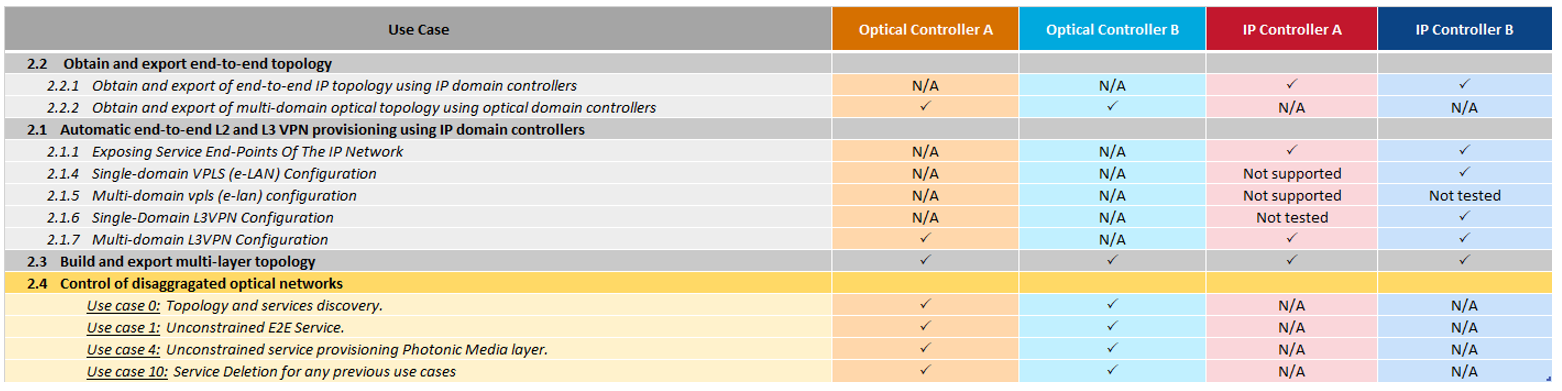
\includegraphics[scale=0.5]{figs/tested_use_cases.png}
%	\label{TAB:tested_use_cases}
%\end{table*}

%\subsection{Multi-layer Topology Discovery \& Visualization}
%Obtaining the end-to-end multi-layer and multi-domain topology via automatic network discovery is considered the starting point towards the deployment of the SDTN multi-layer solution in the network scenario described in Section 5. The first and most important step is for SDTN to discover all the network elements of the different domains by using the APIs provided by each of the IP and Optical Controllers, as described in previous sections. 

%Technically talking, the following steps take part of the end-to-end network discovery procedure:
%\begin{enumerate}
%    \item \textit{Enabling Network Adapters}: The network for each domain was discovered from the domain controllers individually by using Domain Adapters; each adapter uses the API provided by the Domain Controller to retrieve data such as nodes, inventories, termination points, links and services within it.
%    \item \textit{Data Model Mapping}: The information model used in the Domain Controller's API is mapped into the SDTN model in order to harmonize the data across all domains, providing both a per-layer view within the inter-layer links and client-server relationships, thus resulting in a complete multi-layer view of the network and its services.
%    \item \textit{Inter-domain links discovery}: End-to-end view of the whole network topology is formed by discovering the inter-domain links. Those interconnect the different vendors into a whole end-to-end multi-layer and multi-domain topology. There are many different mechanisms\footnote{TTI or plug-id for L0/L1, LLDP for L2, IP address based discovery for L3, among others such as alarm/statistics correlation with or without test data/circuits, inter-domain links simulation if no automatic mechanism is available} 
%    to achieve this purpose, such as TTI for OTU links, IP addresses for IP links etc. If all the data required for full inter-domain and inter-layer link discovery is not reported by the third-party controllers, external data can be fed in via the SDTN NBI. 
%\end{enumerate}

%The number of discovered elements within the end-to-end network topology is summarized in \ref{TAB:discovered_elements}, for the optical domains in particular, the number of nodes for each topology correlates to the different layers such as:
%PHOTONIC\_MEDIA LAYER, DSR LAYER and ODU LAYER as defined in the YANG data model for T-API 2.1, hence the reason why there are more nodes retrieved other than those which are physically implemented in the testbed scenario. Additionally, the service interface points (SIPs) discovered for the Optical Domain are exposed in the Controllers NBI, making it easier for the SDTN to access these parameters and using them for future service provisioning. 

%In the IP domain however, given the different models implemented on the IP Controllers, the service end-points were not exposed to the SDTN SBI, reason why the interfaces and ports were needed to be configured manually via Python scripting, being this a drawback when it comes to working with models which don’t follow a fully standardized model.

%\begin{table*}[]
%\caption{Discovered Network Elements for the Topology Visualization}
%\begin{adjustbox}{width=1\textwidth}
%\small
%\begin{tabular}{lllll}
%\hline
%{\color[HTML]{000000} } &
%  {\color[HTML]{000000} Optical Controller A} &
%  {\color[HTML]{000000} Optical Controller B} &
%  {\color[HTML]{000000} \begin{tabular}[c]{@{}l@{}}IP Controller A\end{tabular}} &
%  {\color[HTML]{000000} IP Controller B} \\ \hline
%{\color[HTML]{000000} \begin{tabular}[c]{@{}l@{}}Discovered nodes \\    (physical and logical)\end{tabular}} &
 % {\color[HTML]{000000} 17} &
%  {\color[HTML]{000000} } &
%  {\color[HTML]{000000} 11} &
%  {\color[HTML]{000000} 13} \\
%{\color[HTML]{000000} \begin{tabular}[c]{@{}l@{}}Discovered links\\    (physical and logical)\end{tabular}} &
%  {\color[HTML]{000000} 18} &
%  {\color[HTML]{000000} } &
%  {\color[HTML]{000000} 13} &
%  {\color[HTML]{000000} 15} \\
%{\color[HTML]{000000} Discovered service-end-points\footnote{The amount of end-points discovered for the domains not only comprehend those available for service provisioning, but all those available in the network }} &
%  {\color[HTML]{000000} 97} &
%  {\color[HTML]{000000} 90} &
%  {\color[HTML]{000000} Not automatically discovered} &
%  {\color[HTML]{000000} Not automatically discovered} \\
%\rowcolor[HTML]{EFEFEF} 
%{\color[HTML]{000000} Intra-domain IP links} &
%  \multicolumn{4}{c}{\cellcolor[HTML]{EFEFEF}{\color[HTML]{000000} 2}} \\
%{\color[HTML]{000000} Intra-domain Optical links (automatically discovered)} &
%  \multicolumn{4}{c}{{\color[HTML]{000000} 4}} \\
%\rowcolor[HTML]{EFEFEF} 
%{\color[HTML]{000000} \begin{tabular}[c]{@{}l@{}}Inter-layer Inter-domain links
%\end{tabular}} &
%  \multicolumn{4}{c}{\cellcolor[HTML]{EFEFEF}{\color[HTML]{000000} 8}} \\ \hline
%\end{tabular}
%\end{adjustbox}
%\label{TAB:discovered_elements}
%\end{table*}

%\subsection{Single-domain IP L2VPN provisioning}
%
%This use case has been tested using a single IP Controller and using the L2SM model to request the service creation between the SDTN and the IP SDN controller. The process for the L2VPN service creation is described in the following steps:
%
%\begin{enumerate}
%    \item Site creation. The two sites must be created on the SDN-C. Parameters such as \texttt{site-id} and \texttt{location-id} must be provided.
%    \item Service Creation. Virtual Circuit Identifier \texttt{VC-ID} to be negotiated by the ends is provided.  
%    \item Site Network Access Creation (SNA). In this step all the data previously created is merged together into a working L2VPN service to be deployed by the SDN-C on the devices using NETCONF. The configuration parameters needed on the body request for the SNA creation includes \texttt{site-id}, \texttt{bearer-id} and \texttt{vpn-id}, among others such as IP connectiviy, QoS management or Ethernet encapsulation. 
%\end{enumerate}

%\begin{figure}
%	\centering
%		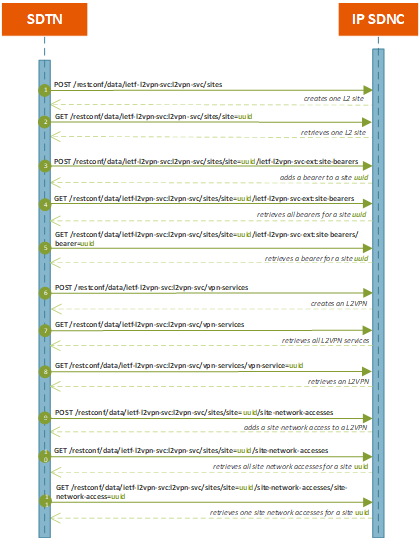
\includegraphics[width=\linewidth]{figs/l2sm_workflow_2.png}
%	\caption{Messages Interchanged for L2VPN Provisioning between the SDTN and the IP SDN-C}
%	\label{FIG:L2SM_workflow}
%\end{figure}

%The workflow between the SDTN and the IP Controller has been summarized in the UML model presented on \ref{FIG:L2SM_workflow}. The four POST requests described previously and their equivalent GET requests exchanged between the SDTN and the IP-SDN controller are included. \ref{FIG:L2SM_results} shows the L2VPN service creation results as seen from the SDTN GUI, where three information panes are included: 
%\begin{itemize}
%    \item Configured NEs in the network map. The yellow ones include the two service end-points.
%    \item List of all the services of a common type. In this case VPLS service was selected. 
%    \item Service details, including: Name, Description and End-points (vlans, ports and topology-role). 
%\end{itemize}

%\begin{figure}
%	\centering
%		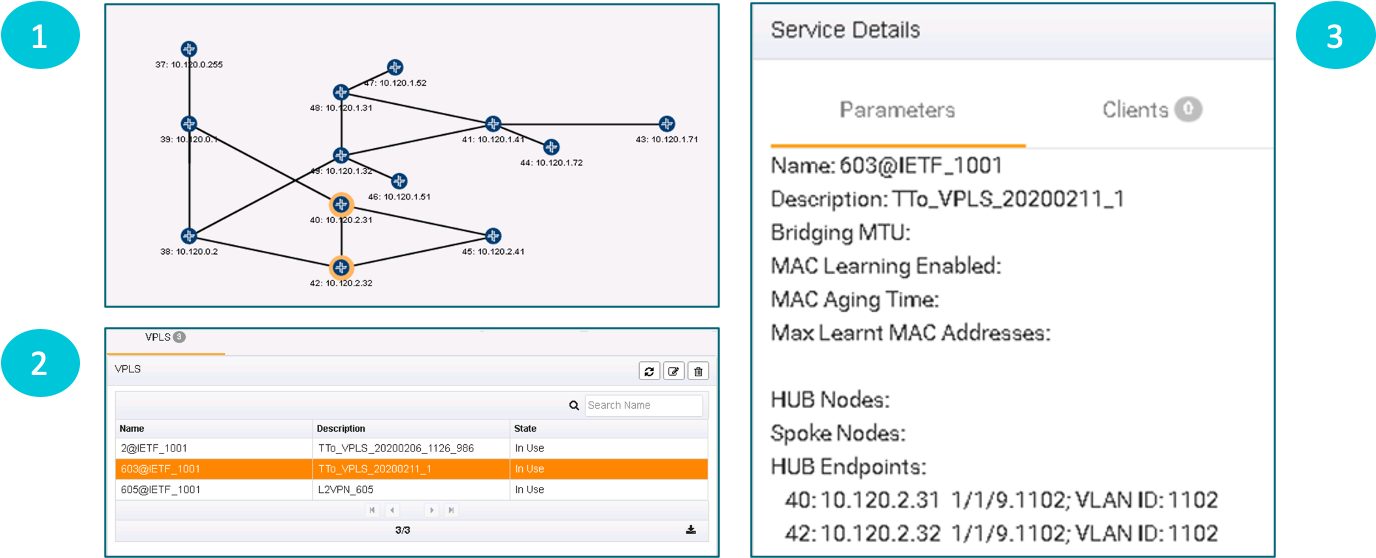
\includegraphics[width=\linewidth]{figs/l2vpn_results.png}
%	\caption{L2VPN service creation results retrieved from the SDTN GUI. Information included three panes: Topology, Services lists and Service Details (Name, Topology and Endpoints).}
%	\label{FIG:L2SM_results}
%\end{figure}


\subsection{Multi-domain IP L3VPN provisioning}

This section presents the test results for the Hierarchical SDTN Controller integration with the controllers in the IP/Optical domains. Two types of tests have been done to demonstrate orchestration functionalities in the multi-layer/multi-domain/multi-vendor network environment, as depicted in \Cref{FIG:testing_workflow}. In a first stage, each \replaced{SDNc}{SDN controller} was validated individually. RESTCONF-based queries were sent towards each of the SDNCs to change and retrieve the network information and validate each implementation's compliance. This initial certification aimed to make functional tests over each solution and speed-up the entire solution's final integration. The scalability and efficiency of the SDTN \added{Controller} solution is limited to the SDNc performance.

\begin{figure}
	\centering
		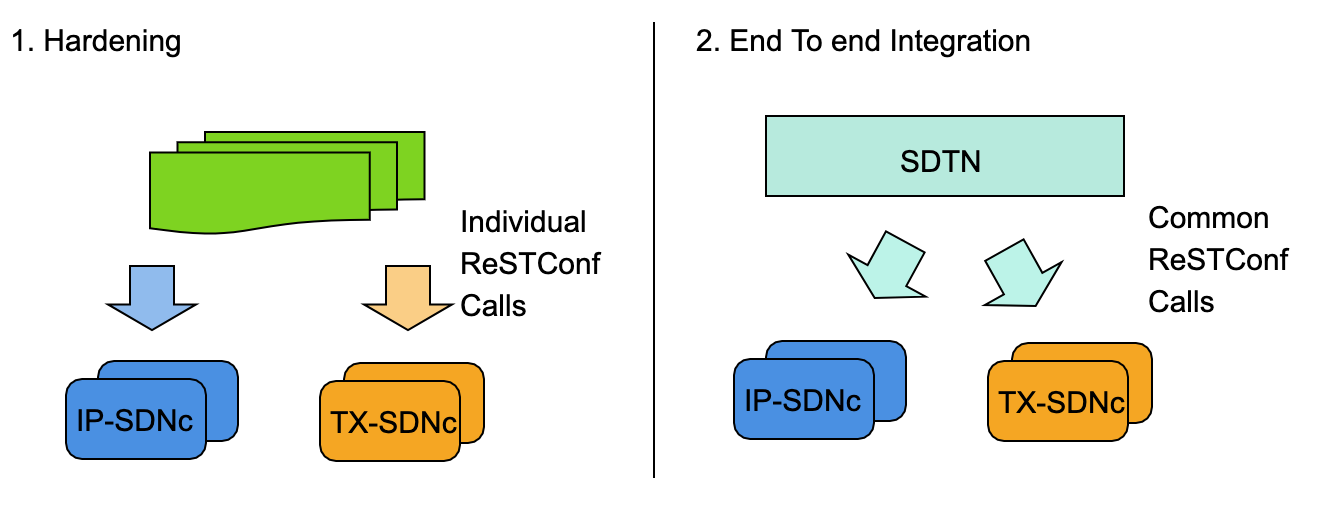
\includegraphics[width=\linewidth]{figs/diagram-11.png}
	\caption{The two types of tests have been done in order to demonstrate orchestration functionalities in the multi-layer/multi-domain/multi-vendor network environment. (1) Hardening process includes single domain tests. (2) End to end integration includes the SDTN \added{Controller} delegation of resources to the domain controllers.}
	\label{FIG:testing_workflow}
\end{figure}

\begin{figure*}
	\centering
		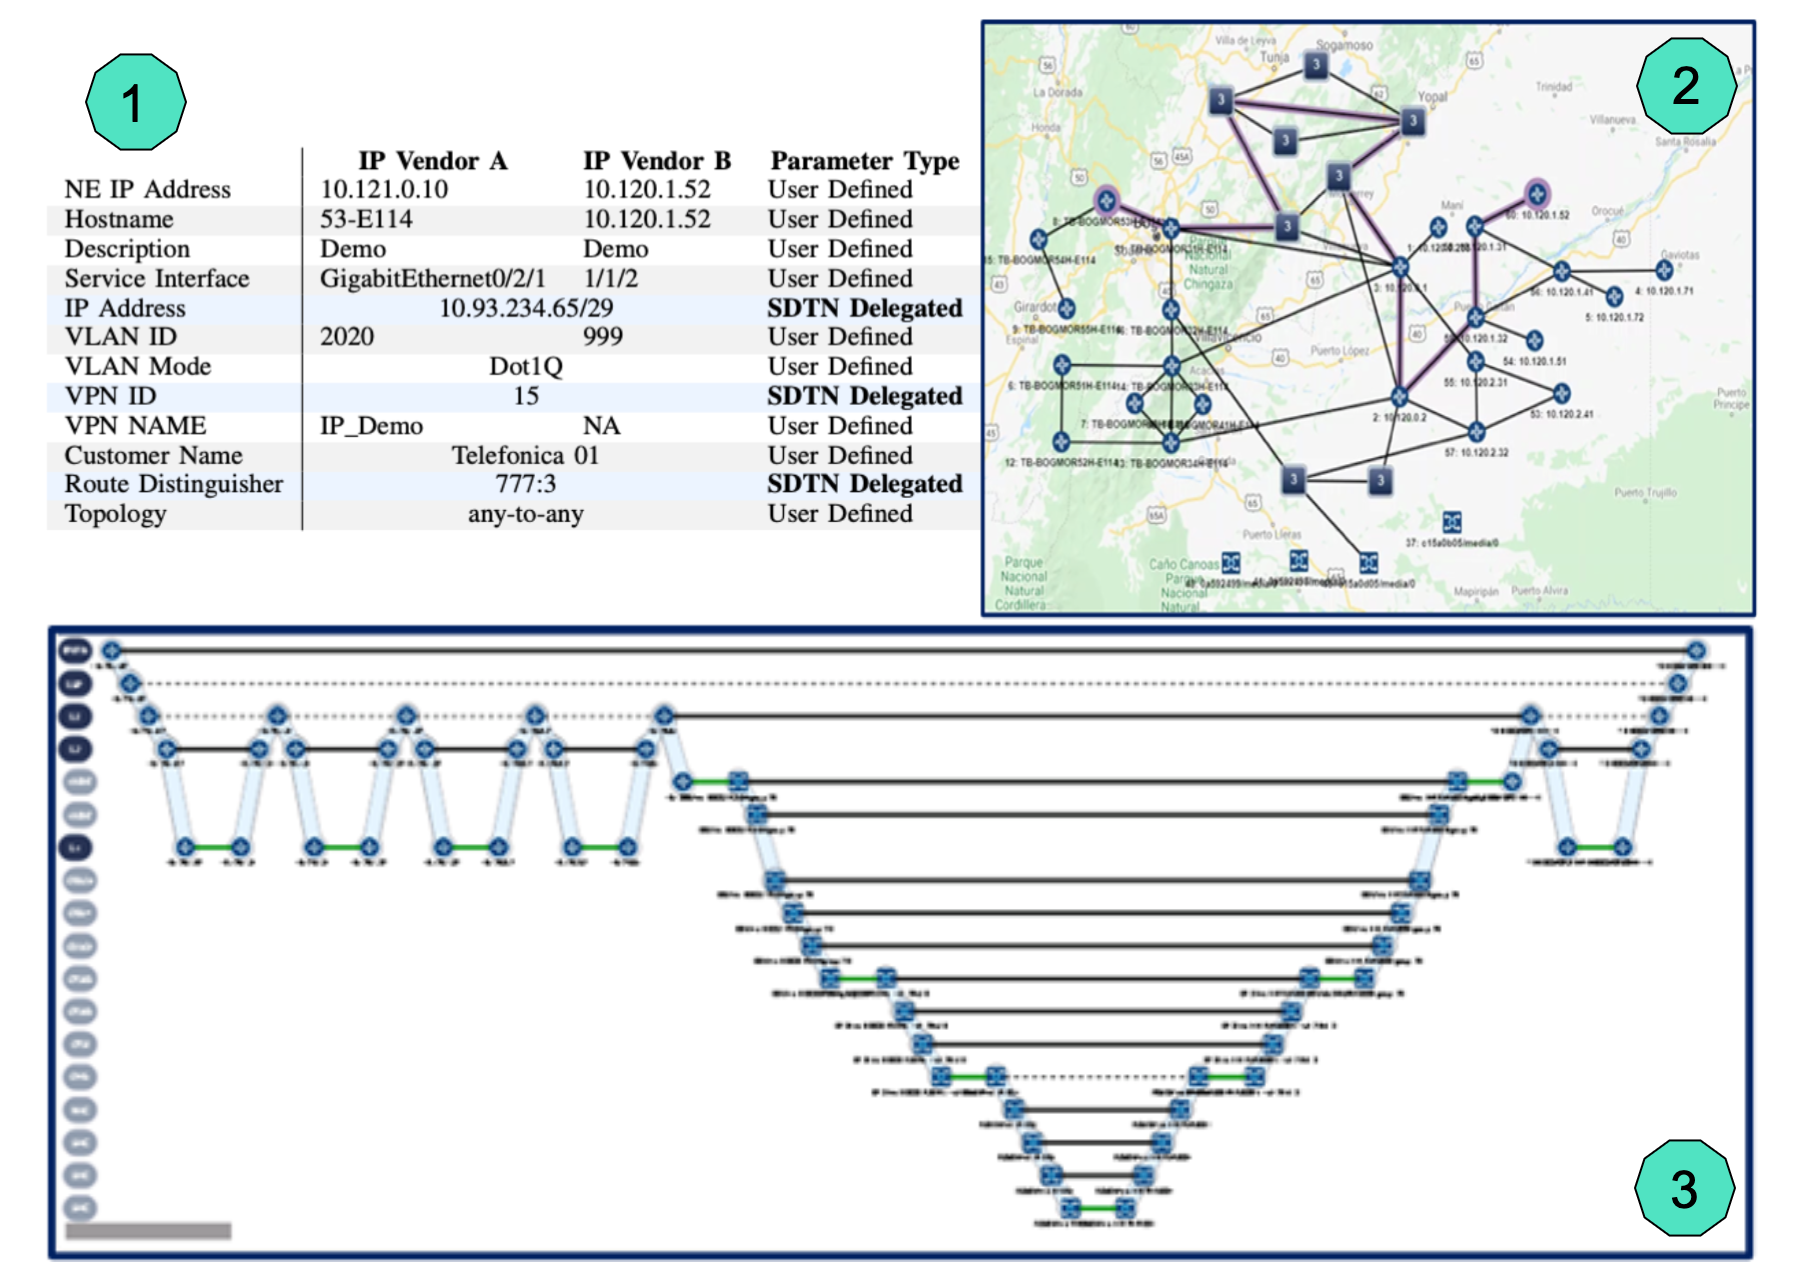
\includegraphics[width=\linewidth]{figs/diagram-14.png}
	\caption{L3VPN service creation results retrieved from the SDTN \added{Controller} GUI. Included three visualization panes: The service details (Name, Topology, RD and Endpoints), the geographical view and the hop-by-hop connection view.}
	\label{FIG:l3vpn_results}
\end{figure*}


Once each domain controller was independently certified during the individual validation process, the end-to-end integration was done using multi-domain functional tests. In that case, the Transcend Meastro GUI was used to orchestrate the entire service lifecycle. For example,  to create a service between two domains, the SDTN \added{Controller} provided a Graphical template to fill the service creation parameters. The parameters depicted in \Cref{FIG:l3vpn_results} includes the user-defined configuration requirements and the auto-assigned parameters by the SDTN \added{Controller}. In both cases, the SDTN \added{Controller} stored the whole service resources, and It continuously monitors the network state to keep the set of values synchronized. The workflow used is by the SDTN is depicted in \Cref{FIG:l3vpn_workflow}. Each time a user created a service, a set of request calls was instantiated between the SDTN \added{Controller} and the corresponding SDNc. Finally, once the SDNc confirms the service creation to the SDTN \added{Controller}, the Transcend Maestro provided three visualization options: (1) Service details, (2) Geographical view, and (3) Layered view, as depicted in \Cref{FIG:l3vpn_results}.

%Aiming to demonstrate the multi-domain/multi-vendor capabilities of the SDTN solution, a scenario for an L3VPN service configuration was proposed. The main goal was to create a L3VPN between two access routers, each of them located in different IP domains. The IP domains are connected using a DWDM optical network. The L3VPN service was created using the SDTN GUI and the configuration parameters used for this matter are shown on Table \ref{TAB:discovered_ip_l3vpn}.
%The workflow between the SDTN and the IP Controller for the l3vpn creation has been summarized in the UML model presented on \cref{FIG:testing_workflow}. 

\begin{enumerate}
    \item The VPN service details including the service name, the topology and end-points. 
    \item The service route in the topology view, this view includes the full path including the IP and Optical devices compromised in the service.
    \item Layered view of the service. This view splits the service connections between layers, so the IP Links connection is in the top. The Ethernet connections between routers are in the second layer and physical plus optical layers are decoupled in this hierarchical structure.
\end{enumerate}

\begin{figure*}
	\centering
		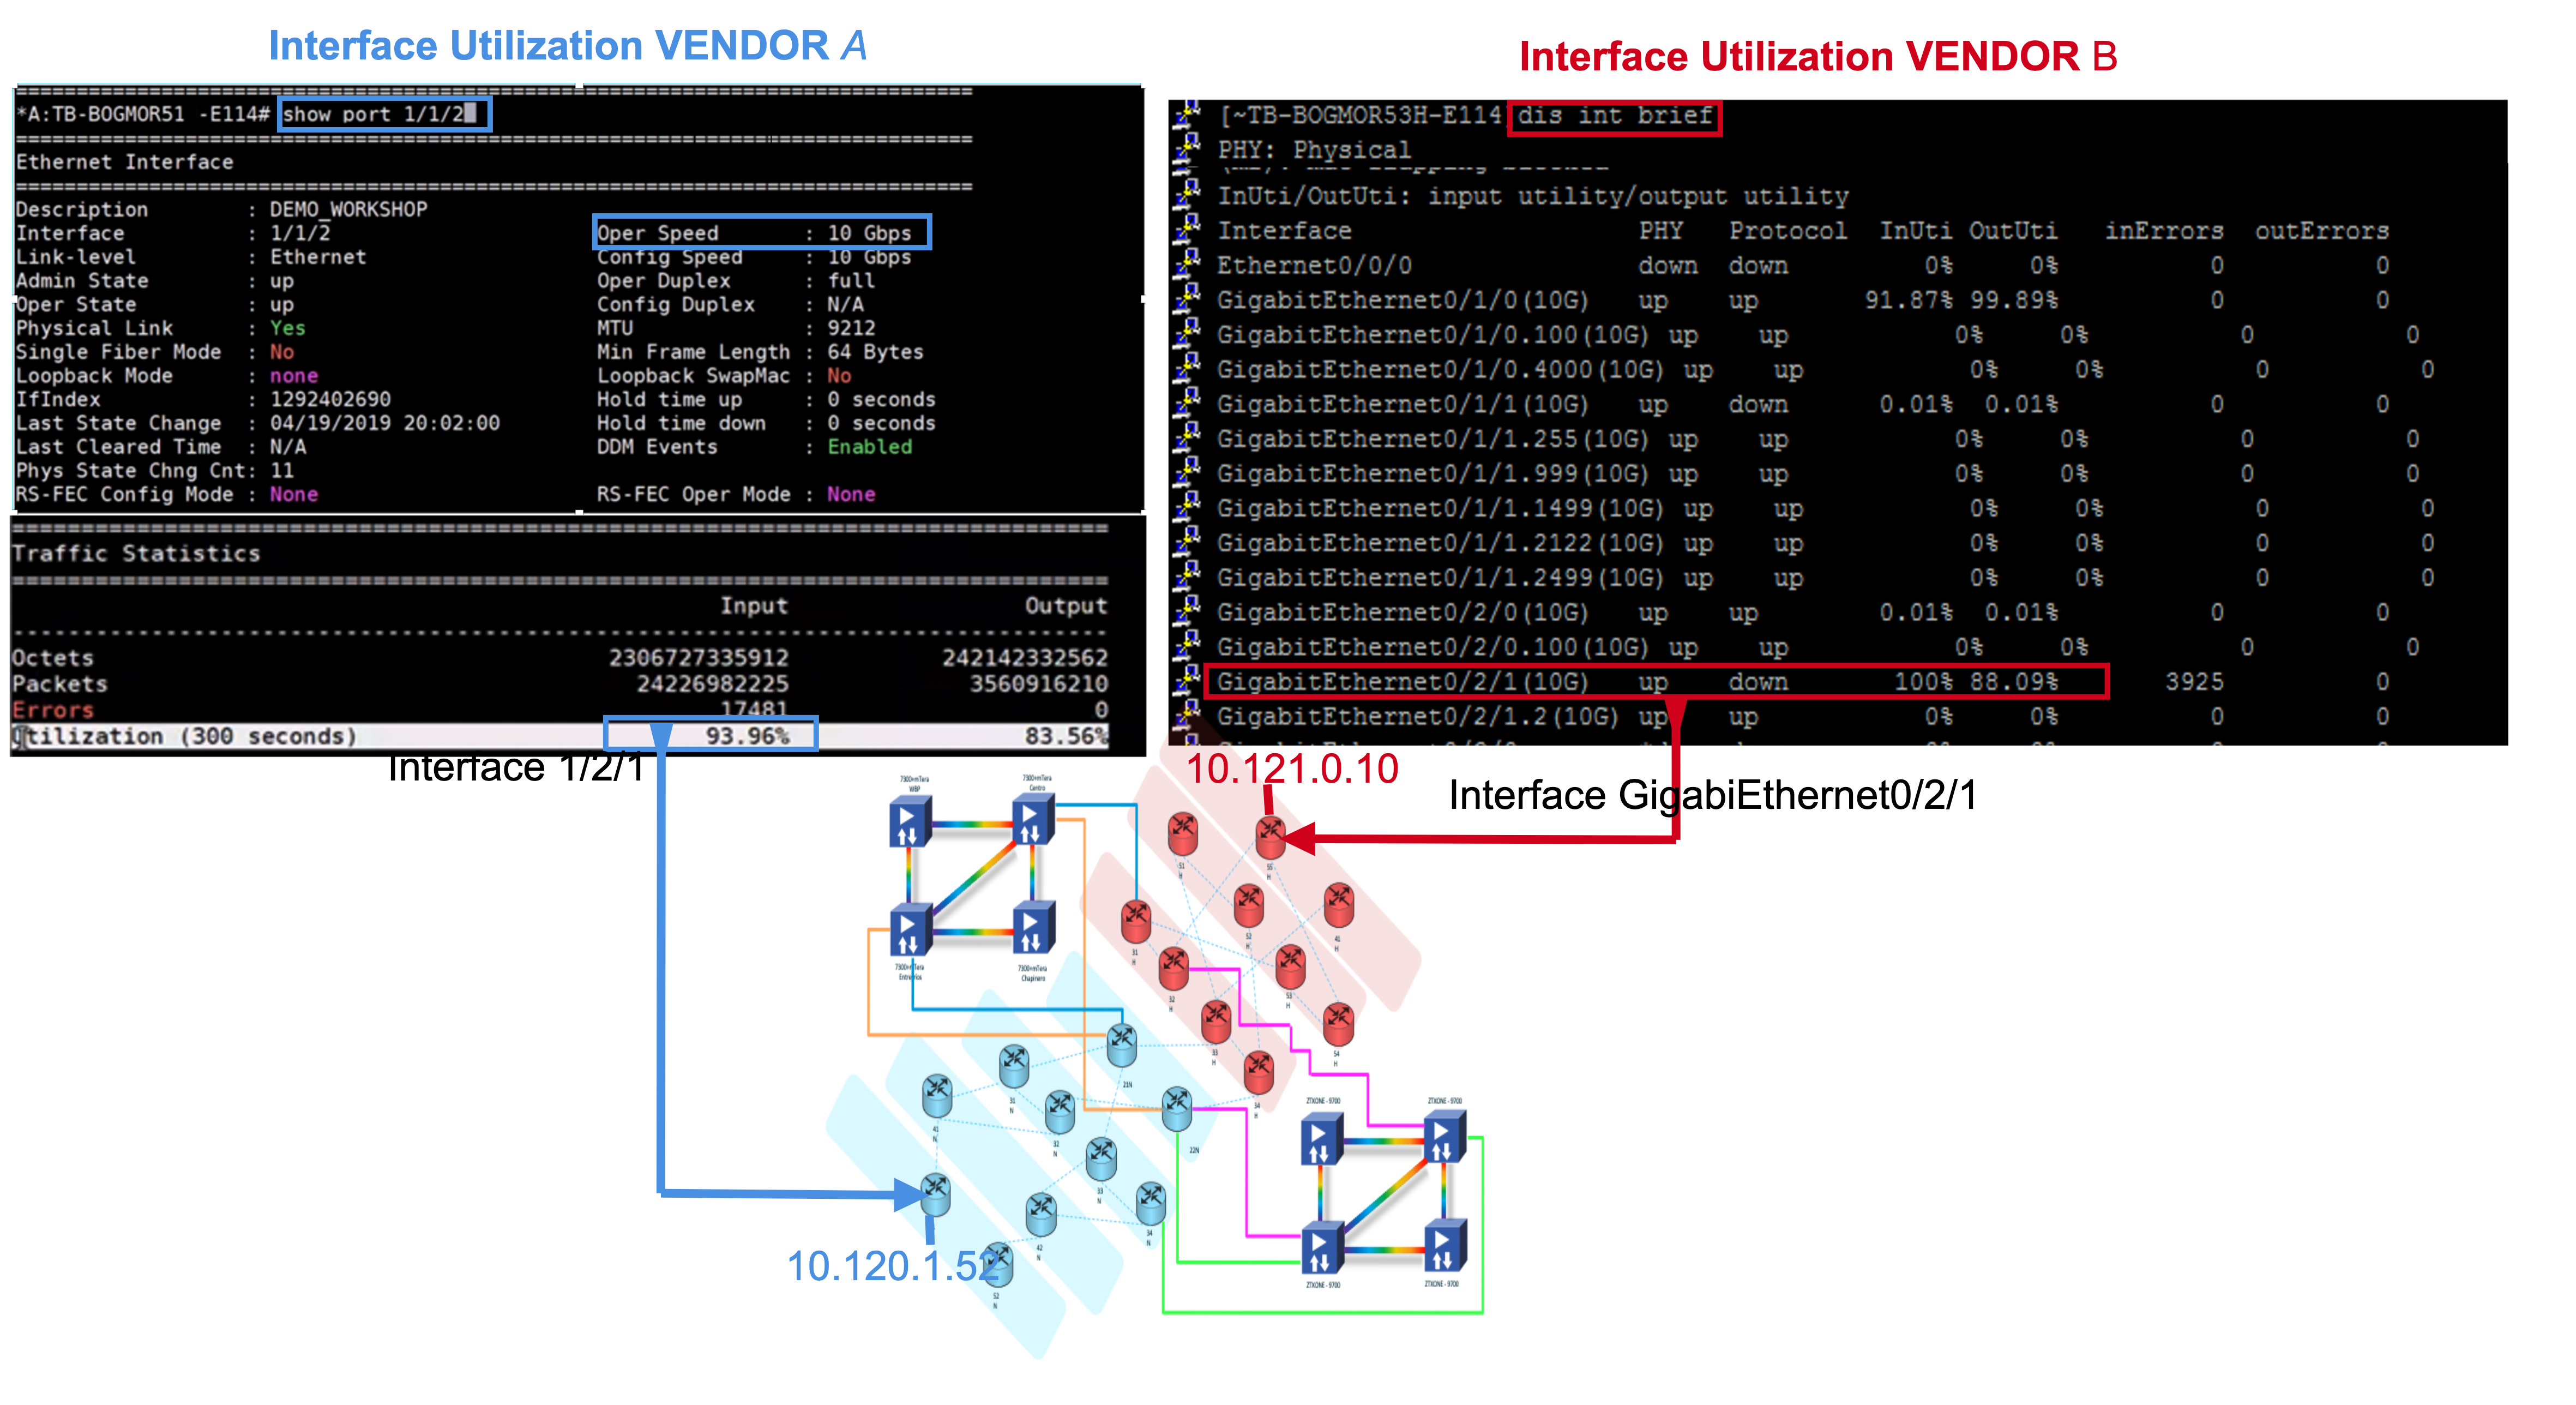
\includegraphics[width=\linewidth]{figs/counters1.png}
	\caption{Traffic counters measured on the end-points of the service. The utilization in both ends is close to 95\% due to the traffic injected by the generator.}
	\label{FIG:counters}
\end{figure*}

% \begin{table}[]
% \caption{Configuration Parameters for the testing of the L3VPN}
% \label{TAB:params}
% \begin{adjustbox}{width=0.5\textwidth}
% \small
% \begin{tabular}{l|lll}
% & \multicolumn{1}{c}{\textbf{IP Vendor A}} & \multicolumn{1}{c}{\textbf{IP Vendor B}} & \multicolumn{1}{c}{\textbf{Parameter Type}}\\
% {\color[HTML]{000000} NE IP Address} & {\color[HTML]{000000} 10.121.0.10}          & {\color[HTML]{000000} 10.120.1.52}   & {\color[HTML]{000000} User Defined}   \\
% \rowcolor[HTML]{F2F2F2} 
% {\color[HTML]{000000} Hostname}            & {\color[HTML]{000000} 53-E114}              & {\color[HTML]{000000} 10.120.1.52}    & {\color[HTML]{000000} User Defined} \\
% {\color[HTML]{000000} Description}         & {\color[HTML]{000000} Demo}      & {\color[HTML]{000000} Demo} & {\color[HTML]{000000} User Defined}\\
% \rowcolor[HTML]{F2F2F2} 
% {\color[HTML]{000000} Service   Interface} & {\color[HTML]{000000} GigabitEthernet0/2/1} & {\color[HTML]{000000} 1/1/2} & {\color[HTML]{000000} User Defined}          \\
% \rowcolor[HTML]{ECF4FF} 
% {\color[HTML]{000000} IP Address}          & \multicolumn{2}{c}{\color[HTML]{000000} 10.93.234.65/29}     & \multicolumn{1}{l}{\color[HTML]{000000} \textbf{SDTN Delegated}}\\
% \rowcolor[HTML]{F2F2F2} 
% {\color[HTML]{000000} VLAN   ID}           & {\color[HTML]{000000} 2020}                 & {\color[HTML]{000000} 999}         & {\color[HTML]{000000} User Defined}    \\
% {\color[HTML]{000000} VLAN Mode}           & \multicolumn{2}{c}{{\color[HTML]{000000} Dot1Q}} & {\color[HTML]{000000} User Defined}                                     \\
% \rowcolor[HTML]{ECF4FF} 
% {\color[HTML]{000000} VPN   ID}            & \multicolumn{2}{c}{{\color[HTML]{000000} 15}} & \multicolumn{1}{l}{\color[HTML]{000000} \textbf{SDTN Delegated}} \\
% {\color[HTML]{000000} VPN NAME}           & {\color[HTML]{000000} IP\_Demo}                 & {\color[HTML]{000000} NA} & {\color[HTML]{000000} User Defined} \\
% \rowcolor[HTML]{F2F2F2}
% {\color[HTML]{000000} Customer Name}            & \multicolumn{2}{c}{\cellcolor[HTML]{F2F2F2}{\color[HTML]{000000} Telefonica 01}} & \multicolumn{1}{l}{\color[HTML]{000000} User Defined}\\
% \rowcolor[HTML]{ECF4FF}
% {\color[HTML]{000000} Route Distinguisher}           & \multicolumn{2}{c}{{\color[HTML]{000000} 777:3}} & {\color[HTML]{000000} \textbf{SDTN Delegated}}\\
% \rowcolor[HTML]{F2F2F2}
% {\color[HTML]{000000} Topology}            & \multicolumn{2}{c}{\cellcolor[HTML]{F2F2F2}{\color[HTML]{000000} any-to-any}} & \multicolumn{1}{l}{\color[HTML]{000000} User Defined}\\
% \end{tabular}
% \end{adjustbox}
% \end{table}


The configuration of the IP L3VPN service in the network elements was verified by using their command line interface as well as the IP\replaced{SDNc}{-SDN controllers} GUI. To validate the data plane, a traffic generator was used in site to introduce traffic on both ends of the network and tested the multi-domain L3VPN service. \Cref{FIG:counters} shows the traffic statistics as seen on the command-line interface of the PE routers. In this figure, the two interfaces connected to the VPN services are selected, and their traffic counters are showed. \replaced{Figure 6 shows the bandwidth utilization of 93.96\% and 88\% on each end of the VPN service.}{The occupancy of the 10G ports is close to the 95\% during the test.} 

%\subsection{Optical provisioning}
%From the perspective of the optical networks, single domain unconstrained DSR connectivity services as well as Photonic Media Layer services were independently configured in both vendors’ DWDM networks and were verified in the respective NMS systems. The ONF T-API 2.1 YANG data model has been used for the query exchange between the SDTN HCO and the optical domain controllers given the support of this standard model in their NBIs. The UML diagram on \ref{FIG:optical_provisioning_workflow} shows the HTTP POST request involved in the optical circuit creation as sent from the SDTN HCO towards the Optical SDNCs, as well as the HTTP GET requests for information retrieval regarding particular connectivity services existing on the network. 

%The DSR connectivity services created in both optical domains range from 1GbE, to 10GbE and 100GbE, all of them configured by using the API Client as well as the SDTN HCO GUI. A total of 3x10GbE and 4x100GbE DSR connectivity services were provisioned simultaneously on Optical Domain A whereas given the network resources available in the Optical Domain B, a 1GbE service as well as 2x10GbE services were provisioned. When it comes to photonic media type of services, 100GbE and 200GbE could be provisioned for Optical Domain A and B respectively. 

%First, the API Client was used to send the E2E DSR Service creation query towards the SDNCs. For this, parameters\footnote{Parameters included in the body script for the service creation; other important ones include \texttt{service-interface-point}, \texttt{layer-protocol-name}, \texttt{service-layer} as well as the \texttt{service name} and a unique identifier \texttt{uuid}.} such as \texttt{service-interface-point}, \texttt{capacity} and the \\ \texttt{layer-protocol-qualifier} embedded in the POST body script needed to be correctly identified prior to sending the service creation petition, being that they depend strictly on the installed equipment and the resources available in the network; and therefore, when configured improperly, it led to the failure of the service creation, or to the misconfiguration on the controller’s side. When sending the POST query from the SDTN HCO towards the Optical Controllers, an HTTP 202 Accepted notification is returned by the SDNC, meaning the controller has accepted the petition and would proceed with the service creation, otherwise, an HTTP 400 Bad Request notification would be retrieved in case the petition was not accepted by the controller. 

%\begin{figure}
%	\centering
%		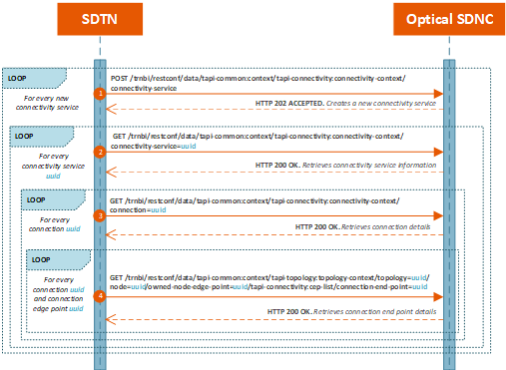
\includegraphics[width=\linewidth]{figs/optical_provisioning_workflow_2.png}
%	\caption{Messages Interchanged for Optical Provisioning between the SDTN and the Optical SDN Controller}
%	\label{FIG:optical_provisioning_workflow}
%\end{figure}

%\begin{figure}
%	\centering
%		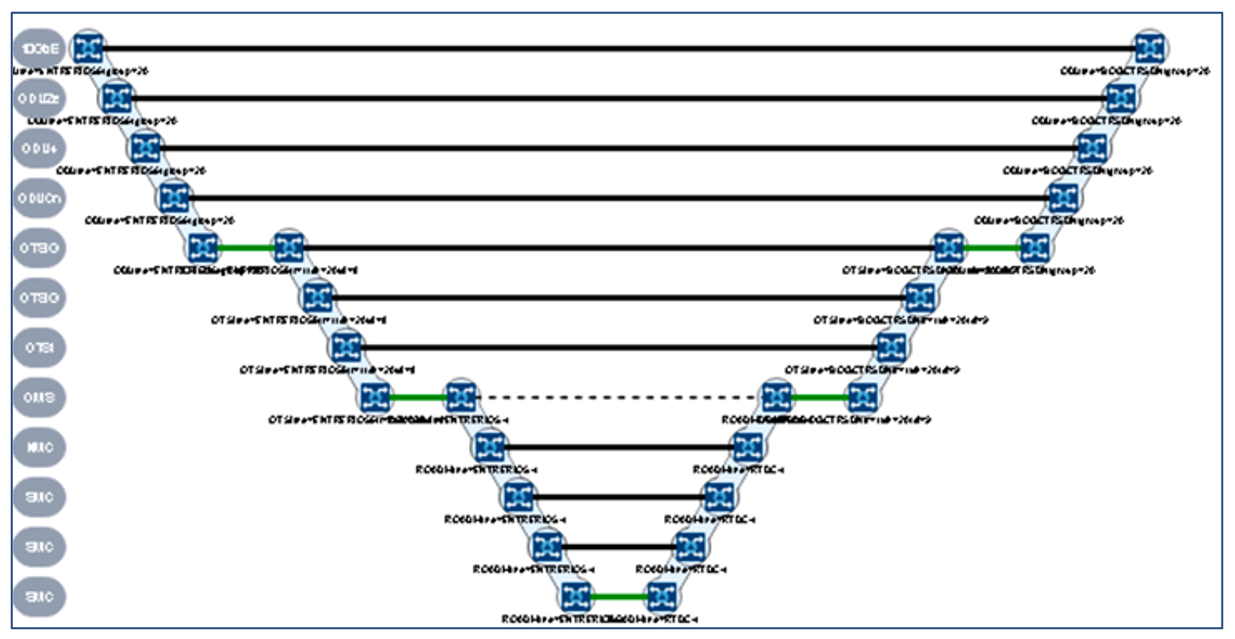
\includegraphics[width=\linewidth]{figs/optical_provisioning_result.png}
%	\caption{Optical Provisioning Result for a Multi-Layer 10GbE Service}
%	\label{FIG:optical_provisioning_result}
%\end{figure}

%Additionally, from the API client tests, it was noted that even if both controllers are standard-based and implement T-API 2.1 in their NBIs, the modelling of some attributes is different from one another. From comparing the results retrieved via the API Client, naming attributes for some of the objects\footnote{SIP\_NAME” in contrast to "INVENTORY\_ID", "CONN\_NAME" in contrast to "CONNECTION\_NAME", among others}, as well as the general modelling of the connections in regards of the route for an optical circuit was noticed to be different. Likewise, the site names in one of the optical controllers did not coincide with the real name of the site but were based on an encoding made it by the controller itself. Also, when using the SDTN HCO GUI to create the e2e connectivity services within the two network domains; this particular discrepancy was also visible via the multilayer view of the services created, as seen on \ref{FIG:optical_provisioning_workflow} where the different layers for a 1GbE service are shown as exposed by the optical domain controller B, while on \ref{FIG:optical_provisioning_result} a multilayer view of 10GbE service created on Optical Controller A is shown.


\section{Conclusions and Future Work}
\label{section:conclusions}
%A key angular stone for the SDTN Architecture is the data models themselves. RESTCONF/YANG based with IETF were preferred when beginning with the integration between SDTN and the SDN-Cs, the main focus was the use of a standardized API to access and retrieve the required information from the IP and Optical controllers. The usage of different pseudo-standard and reduced models was needed in order to execute the different test case scenarios. IETF YANG data models for the IP World still require additional efforts to fit in all the MPLS-based use cases as a synergy flow. 

\replaced{It is fundamental for the SDN adoption in service provider networks defining the data models and protocols used across the components.}{A key angular stone for the SDN adoption in service provider networks is the definition of the data models and protocols to be used by the architecture components for the integration between them.} Historically, integration using proprietary interfaces delay the introduction of programmability and automation and have a high economic cost. In this work, RESTCONF with IETF YANG models was tested for the integration between the SDTN \added{Controller} and the IP SDNcs. \added{This work shows, for the first time,} a standardized \added{L3NM} API to provision and retrieve services to a multi-vendor underlay network. \added{Moreover, this paper presents an infrastructure using network elements in the production network of Telefonica Colombia.}

The tests included the provision of L3VPN using IETF YANG data models and the topology collection. The SDTN \added{Controller} orchestrated the service creation assigning the resources to each domain controller. During the service retrieval, the SDTN \added{Controller} composed the services based on the information exposed by the domain controllers.

For additional tasks, there are still gaps to cover all the IP/MPLS network operation requirements. A brief summary of the issues faced during the integration, as reference point to future work are: 

\begin{itemize}
    \item Connectivity, latency and internal processing times between the HCO and some of the SDNcs can impact the integration and result in miscommunications creaking the timeout of SDN transport protocols, ie. RESTCONF and NETCONF.   
    \item \textit{Ghost} objects which would not be completely deleted in the controllers can lead to misunderstand in the topology construction.
    \item The unsolicited data retrieved by a lack of standardization or a bias in the implementation of the standards can lead to uncompleted transactions or loops in execution tasks.
    \item Absence of data in the SDN domain controllers for an automatic inter-domain link discovery.
    \item Differences in the RESTCONF/YANG implementations on the \replaced{SDNc}{SDN Controllers}. Even if the YANG models were the same, the parameters translation between NBI and SBI can restrict some configurable parameters (i.e max length size of a description field) and may generate implementation differences. This would derive in possible errors during the execution of the creation process.
    \item Differences in the RESTCONF/YANG error handling. A set of well defined error codes is mandatory in the hierarchical architecture.
\end{itemize}

%However, except for the lack of the inter-domain ports exposure on the IP domains as well as the retrieval of data required for automatic discovery of Inter-Domain Links (e.g. \texttt{Plug-ID} and TTI values), 

The APIs designed in this work demonstrates the viability of the i\uppercase{FUSION} architecture with an SDTN \added{Controller} orchestrating an underlay multi-vendor, multi-layer, and multi-domain network environment. The i\uppercase{FUSION} APIs allow any service provider to migrate brownfield scenarios into SDN-ready domains using programmatic interfaces.

\subsection{Future Work}
As future work, the hybrid SDN deployment done until now must be complemented with an integration between the NBI exposed by the SDTN \added{Controller} and the OSS applications ecosystem. The OSS ecosystem can include for example strategic and tactical planning applications, able to support the year by year demand management and planning tasks done within the organization. A common interface defined and available for these tasks would allow the OSS systems providers to focus on the quality of the applications developed, forgetting the complexity of the network management. Economically it will generate direct reductions in the applications integration time.

%Additionally, the scope of this work can be extended to cover Traffic Engineering use cases. Standardization in the NBI requests to support the LSPs creation will enable easy management of the traffic flows in the network, generating a real massification of the Traffic Engineering deployment and creating new network optimization solutions for the operators.

\section*{Acknowledgements}
This \deleted{is} work has been supported by Telefonica I+D as part of the Fusion, i\uppercase{FUSION}, OpenFusion projects and partially funded by the EC 5GPPP TeraFlow (101015857) and MINECO AURORAS (RTI2018-099178-B-I00). Authors would like to thank to all the SDN technical teams and leaders that participate in the development, deployment, and testing of this \deleted{SDTN} architecture. Many thanks for their contributions to Manuel Santiago, Gloria Gomez, Julia Rodriguez and Zdravko Stevkovski from Infinera, Randy Quimbay, David Rocha from Telefonica Colombia, and Andrea Valencia, Juan Suarez, Juan Agredo and Daniel Hernandez from Wipro.   

%\bibliographystyle{ieeetr}
\bibliographystyle{IEEEtran}
\bibliography{Biblio}

\begin{IEEEbiography}
[{
\includegraphics[width=1in,height=1.25in,clip,keepaspectratio]{1010179793S.jpg}}]%
{Samier Barguil} (M.Sc. 2018). PhD Candidate from the Universidad Autonoma de Madrid. Electronic Engineer from the District University of Bogot\'a Franscisco José de Caldas and Master in Science in Industrial Automation of the Universidad Nacional de Colombia. Currently is the IP SDN Technical Leader at Wipro Technologies Ltd.\end{IEEEbiography}

\begin{IEEEbiography}[{
\includegraphics[width=1in,height=1.25in,clip,keepaspectratio]{victor.jpg}}]%
{Víctor López} (M.Sc. 2005 - Ph.D. 2009) is a Technology Expert at Systems and Network Global Direction in Telefónica gCTIO. He works on the global IP and transport processes of the Telefonica group. He serves as co-chair at the Open Optical Packet Transport group in the Telecom Infra Project. He has co-authored more than 200 publications, six patents and contributed to IETF and ONF. Moreover, he is the editor of the book Elastic Optical Networks: Architectures, Technologies, and Control (308 pages, Springer 2016). His research interests include the integration of Internet services over IP/MPLS and optical networks and control plane technologies (PCE, SDN, GMPLS).\end{IEEEbiography}

\begin{IEEEbiography}[{
\includegraphics[width=1in,height=1.25in,clip,keepaspectratio]{victor.jpg}}]%
{Cristyan Manta-Caro} (M.Sc. 2007 - PhD (c)) currently serves as Solutions Manager and Managing Consultant at Wipro Technologies Ltd within the Comms EGM BU. He is responsible for structuring and leading transformation projects for Digital and Telecommunications providers. With over 15 years of experience in managing, optimizing, analyzing telecommunications and Information Technology IT infrastructures with primary vendors and CSP. He received his Master of Science and Electronics Engineering degree from the District University of Bogota Francisco Jos\'e de Caldas. His research interests include SDN architectures, Future Internet, DevNet \& NetDevOps, Cloud Technologies for IoT and the Web of Things WoT.\end{IEEEbiography}

\begin{IEEEbiography}Arturo Mayoral López de Lerma is a Technology Expert in Transport Networks at the Global Systems \& Network department of Telefónica GCTIO. He received the Ph.D. degree in telecommunications engineering from the Universitat Politècnica de Catalunya (UPC) in 2019. His  research  interests  include  optical network design and Software Defined Networking (SDN). He is author or co-author on over 50+ journals and conference papers. He graduated in Telecommunications Engineering by the Universidad Autónoma de Madrid in 2013 and he started his professional career in 2012, as undergraduate researcher in Telefonica I+D (R\&D) where developed his Final Career’s Project, awarded with the Best Final Project Prize by the Official College of Telecommunication Engineers (COIT).\end{IEEEbiography}

\begin{IEEEbiography}Oscar González de Dios received his M.S. degree in telecommunications engineering and Ph.D. degree (Hons.) from the University of Valladolid, Spain. He has 19 years of experience in Telefonica I+D, where he has been involved in a number of European research and development projects (recently, STRONGEST, ONE, IDEALIST, and Metro-Haul). He has coauthored over 100 research papers and 10 IETF RFCs. He is currently the head of SDN Deployments for Transport Networks, Telefonica Global CTIO. His main research interests include photonic networks, flexi-grid, interdomain routing, PCE, automatic network configuration, end-to-end MPLS, performance of transport protocols, and SDN. He is currently active in several IETF Working Groups and is the Co-Chair of TIP CANDI WG.\end{IEEEbiography}

\begin{IEEEbiography}Edward Echeverry is Head Of Transport (IP and Optical Network) in Telefonica Colombia. Electronic Engineer, Telecommunications Specialist with a 15+ years of experience in the field. High technical skills and advanced experience in the design, planning and implementation of 3G/4G mobile, IP/MPLS and new generation optical networks, as well as in management and deployment of projects. Lead PoC concept tests of an end-to-end SDTN system including the different layers of IP \& Optical transport network that allowed us to define the use cases of topology and services L1/L2/L3. The tests looked at the use of SBI/NBI T-API IETF-Based interfaces. His research interests include emerging network automation technologies and SDTN architectures.\end{IEEEbiography}

\begin{IEEEbiography}Juan Pedro Fernández-Palacios Giménez received the MS in Telecommunications Engineering from Polytechnic University of Valencia in 2000. In Sept. of 2000 he joined Telefonica I+D where his research activities where focused on the design of new data and control plane architectures for IP over optical networks. He is author of 6 patents filled in Europe and US and more than 70 publications in conferences and journals. He was coordinator of two European research projects on optical transport networks (MAINS and IDEALIST) between 2011 and 2014. In 2013 he joined the Telefonica Global CTO office as Head of Transport. In 2016, he also took this position in Telefonica-O2 Germany. Since June 2017 he is leading the Integrated Transport Centre, a global organization in Telefonica in charge of defining the strategic network planning and technology for IP, DWDM, MW and satellite networks.\end{IEEEbiography}

\begin{IEEEbiography}Janne Karvonen (M.Sc.(Tech.) 1993 Helsinki University of Technology) is a Senior Software Architect at Infinera Corporation. He works in the Systems Architecture Group, focusing on Software Defined Networking Technologies and IP/MPLS Network Management Systems. He has over 30 years of experience in Software Engineering and more than 20 years of experience in Telecommunications Network Management Systems, covering both optical and packet based technologies. His research interests include SDN technologies for multi-layer, multi-domain and multi-vendor networks, with special focus on SDN API technologies, Multi-Layer Path Computation Algorithms and utilization of Machine Learning in SDN networks.\end{IEEEbiography}

\begin{IEEEbiography}Jutta Kemppainen received her Master of Science (Tech.) in 1999 from Helsinki University of Technology (now part of Aalto University). She works as Senior Principal Product Manager at Infinera, managing Infinera multi-layer, multi-domain and multi-vendor transport network automation solutions. She has over 20 years of experience of telecommunications software automation products and has been concentrating on Software-Defined Networking (SDN)-based solutions in the last 7+ years. During this time Kemppainen has been co-operating with 70+ network providers, including many of the largest and technically most advanced in the industry, in designing and defining requirements for practical transport network automation solutions.\end{IEEEbiography}

\begin{IEEEbiography}Natalia Isabel Maya Perfetti is an Electronics and Telecommunications engineer graduated from Universidad del Cauca, Colombia back in 2018; thence, she has been working as a network planning engineer in Infinera Colombia where she supports different tasks related to DWDM Network Planning. For the last year she has also been responsible for the testing of the SDTN solution in the field trial environment.\end{IEEEbiography}

\begin{IEEEbiography}Ricard Vilalta (Girona, 1983) graduated in telecommunications engineering in 2007 and received a Ph.D. degree in telecommunications in 2013, both from the Universitat Politècnica de Catalunya (UPC), Spain. He joined CTTC in 2010, and he is a senior researcher in the Optical Networks and Systems Department. He is an active contributor in several standardization bodies such as ONF (OTCC), ETSI (NFV, ZSM), and IETF (CCAMP, TEAS). He is also a member of the technical steering team of Open Transport Configuration \& Control in ONF. He is leading open source contributions and features in ETSI Open Source MANO (OSM) with special focus on 5G technologies.\end{IEEEbiography}


\end{document}